% = = = = = = = = = = = = = = = = = = = = = = = = = = = = = = = = = = = = = = = = = = = = =
% P  R  E  A  M  B  L  E
% = = = = = = = = = = = = = = = = = = = = = = = = = = = = = = = = = = = = = = = = = = = = =
\documentclass[10pt, twocolumn]{article}
\usepackage{array, amsmath, amssymb}
	\newcolumntype{C}{>{$}c<{$}} % math-mode version of "c" column type
	\newcolumntype{L}{>{$}l<{$}} % math-mode version of "c" column type
\usepackage{array}
\usepackage{booktabs}
\usepackage{bm}
\usepackage[small,labelfont=bf,up,justification=justified,singlelinecheck=false]{caption}
\usepackage{fancyhdr}
\usepackage[bottom]{footmisc}
\usepackage[margin=0.1in]{geometry}
\usepackage{graphicx}
\usepackage{hyperref}
	\hypersetup{
		colorlinks,
		citecolor=black,
		filecolor=black,
		linkcolor=black,
		urlcolor=black
		linktocpage=true,
		linktoc=all,     %set to all if you want both sections and subsections linked
	}
\usepackage[sc]{mathpazo}
\usepackage{mathrsfs}
\usepackage{mathtools} 
\usepackage{marvosym} % silly bullet-point symbols (misc symbols)
\usepackage{microtype} % needed for some reason
\usepackage{multicol}
\usepackage{Needspace}
\usepackage{paralist}
\usepackage{setspace}
	\onehalfspacing 
\usepackage[compact]{titlesec} 			% compact shrinks whitespace around section headings.
\usepackage{verbatim}

% Muh packagez :)
\usepackage{../Packages/ClassCommands}
\usepackage{../Packages/BrandonColors}

\usepackage[breakable, theorems, skins]{tcolorbox}
\tcbset{enhanced}
\tcbuselibrary{xparse}
\RequirePackage{xcolor}


\DeclareRobustCommand{\mybox}[2][gray!20]{%
	\begin{tcolorbox}[   %% Adjust the following parameters at will.
		breakable,
		left=0pt,
		right=0pt,
		top=-13pt,
		bottom=0pt,
		colback=#1,
		colframe=#1,
		width=0.45\dimexpr\textwidth\relax,
		enlarge left by=0mm,
		boxsep=1pt,
		arc=0pt,outer arc=0pt,
		]
		#2
	\end{tcolorbox}
}
\newcommand\graybox[1]{ \mybox[gray!20]{\begin{align}#1\end{align}} }

\newcommand\myfig[2][0.3\textwidth]{\begin{figure}[h!]\centering\includegraphics[width=#1]{#2}\end{figure}}
\newcommand{\myspace}{\vspace{3\bigskipamount}}
\newcommand\p{\Needspace{10\baselineskip} \noindent}

% Muh physix commandz
\newcommand\rhat{\hat r}
\newcommand\thetahat{\hat \theta}
\newcommand\phihat{\hat \phi}
\newcommand\s{\mathcal{S}}
\newcommand{\phidot}{\dot{\phi}}
\newcommand{\rdot}{\dot{r}}
\newcommand{\rddot}{\ddot{r}}
\newcommand\ddphi[1]{\deriv{#1}{\phi}}
\newcommand\ddt[1]{\deriv{#1}{t}}
\newcommand\tlab[1]{\tag{#1}\label{#1}}

% Twocolumn setttings.
\setlength{\parskip}{0.3pt}
\setlength{\columnsep}{1cm}		% space between columns
\setlength{\columnseprule}{0.2pt}
\setlength\tabcolsep{0.2cm}
\renewcommand{\arraystretch}{1.5}	% vertical spacing between tables

% Title header settings.
\renewcommand{\thesection}{\Roman{section}}
\titleformat{\section}[block]{\centering\Huge\scshape}{\thesection.}{1ex}{}
\titleformat*{\subsection}{\centering\Large\scshape}
\titleformat*{\subsubsection}{\centering\large\scshape}

\newcommand\sexin[1]{\section{\protect\hyperlink{sec:\thesection}{#1}}\addtocontents{toc}{\protect\hypertarget{sec:\thesection}{}}}


% Title
\title{\vspace{-10mm}\fontsize{24pt}{8pt}\selectfont\textbf{Analytic Mechanics Notes}\vspace*{-4mm}}
% Author
\author{Brandon McKinzie}
% Date
\date{}

% --------------------------------------------------------------
% --------------------------------------------------------------

\begin{document}
\twocolumn[
\begin{@twocolumnfalse}
\maketitle
\thispagestyle{fancy}
\end{@twocolumnfalse}]

	
	
\addtocontents{toc}{\protect\hypertarget{toc}{}}
\tableofcontents\label{toc}
\clearpage




\twocolumn[
\begin{@twocolumnfalse}
%\maketitle
%\thispagestyle{fancy}
\sexin{Energy (Ch. 4)}
\end{@twocolumnfalse}]

\fontsize{10}{10.2}
\selectfont

% ==================================================================
%===================================================================
% CHAPTER 4 - (Condensed) Energy
% ==================================================================
% ==================================================================
\subsection{\green{Kinetic Energy and Work}}
\begin{itemize}
	\item Basic facts for particle mass $m$ speed $v$:
	\begin{align}
		T &= \onehalf mv^2 \\
		\deriv{T}{t} &= m \dot{\bm{v}}\cdot\bm{v} = \F \cdot \bm{v} \\
		\mathrm{d}T &= \F \cdot d\R \\
		\Delta T &= \int_1^2 \F \cdot \mathrm{d}\R \equiv W(1 \rightarrow 2)
	\end{align}
	where the last equation is the \blue{Work-KE theorem}: the change in $T$ between two points on its path equals the work done by the \textbf{net} force as it moves between the two points. 
\end{itemize}

\subsection{\green{Potential E/Conservative F}}
\begin{itemize}
	\item To define $U(\R)$ corresponding to a given conservative force, first choose reference point $\R_0$ at which $U$ defined to be zero. Then \mybox[gray!20]{
		\begin{align} \tag{4.13}
			U(\R) \equiv -W(\R_0 \rightarrow \R) \equiv -\int_{\R_0}^{\R} \F(\R') \cdot \mathrm{d}\R'
		\label{4.13}
		\end{align}}
	\item Principle of \blue{Conservation of Energy} for One particle:
	\begin{quote}
			If all the $n$ forces $\F_i$ acting on a particle are conservative, each with its corresponding potential energy $U_i(\R)$, the \textbf{total mechanical energy} defined as
			\begin{align}
				E \equiv T + U \equiv T + U_1(\R) + \cdots + U_n(\R)
			\end{align}
			is constant in time.
	\end{quote}
	\item For some general scalar multivariable function $f$, the change in $f$ resulting from a small displacement d$\R$ is just
	\begin{align}
		df = \nabla f \cdot \mathrm{d}\R
	\end{align}
	\item Remember that if any $\F$ is conservative that $\nabla \times \F = 0$. 
\end{itemize}

\subsection{\green{2-Particle Interaction}}
\begin{itemize}
	\item Interaction force only a function of $\R_1 - \R_2$, i.e.\footnote{Notation: $\F_{12}$ is force on particle 1 by particle 2.}
	\begin{align}
		\F_{12} = \F_{12}(\R_1 - \R_2)
	\end{align}
	and so we can learn almost everything about $\F_{12}$ by \textit{fixing $\R_2$ at any convenient point.}
	\item How to take gradients/relationship with Newton's third law:
	\begin{align}
		\F_{12} &= -\nabla_1 U(\R_1 - \R_2) \\
		\nabla_1 U(\R_1 - \R_2) &= -\nabla_2 U(\R_1 - \R_2) \\
		\F_{21} &= -\nabla_2 U(\R_1 - \R_2)
	\end{align}
	\item Total energy $E = T_1 + T_2 + U$ is conserved\footnote{$U$ only included once since it apparently "takes both of [the kinetic energy terms] into account."}. 
	\item Using math and the KE theorem, we can get
	\begin{align}
		W_{tot} = -d\R \cdot \nabla U(\R) = -dU
	\end{align}
	as the total work done: the work done by $\F_{12}$ during $d\R_1$ plus the work done by $\F_{21}$ during $d\R_2$. 
\end{itemize}


% ==================================================================
%===================================================================
% CHAPTER 5 - OSCILLATIONS
% ==================================================================
% ==================================================================
\clearpage
\twocolumn[
\begin{@twocolumnfalse}
	\sexin{Oscillations (Ch. 5)}
\end{@twocolumnfalse}]


\subsection{\green{Hooke's Law}}
\begin{itemize}
	\item Force exerted by a spring (1D):
	\begin{align}
		F_x(x) &= -kx
	\end{align}
	where $x$ is displacement from equilib. $k > 0$ and so \blue{stable equilibrium}. 
	\item Equivalent way to state Hooke's law:
	\begin{align}
		U(x) &= \frac{1}{2} k x^2
	\end{align}
	which can be obtained from expanding $U(x)$ in Taylor series:
	\begin{align}
		U(x) &= U(0) + U'(0) x + \frac{1}{2} U''(0) x^2 + \cdots \\
		&= U'(0) x + \frac{1}{2} U''(0) x^2  \\
		&= \frac{1}{2} U''(0) x^2  
	\end{align}
	
	% ------------------- figure ----------------------
	\begin{figure}[b!]
		\centering
		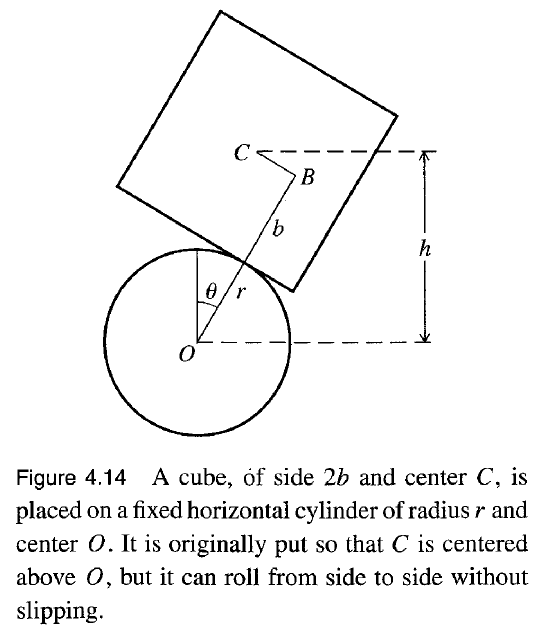
\includegraphics[width=0.4\textwidth]{CubeOnCylinder.PNG}
		\caption{}
		\label{CubeOnCylinder}
	\end{figure} \newpage
	
	\item \purple{\textbf{Example 4.7/5.1}}: Cube balanced on a cylinder (figure ~\ref{CubeOnCylinder})

		
	\begin{itemize}
		\item Clarifications/confusions:
		\begin{itemize}
			\item CYLINDER IS FIXED. In all ways possible. The \emph{cube} can rock back and forth (because apparently it is sentient) but the cylinder itself does not rotate. 
			\item The angle $\theta$ is referring to the angle the cube has rotated. 
			\item Author claims that BC is ''distance the cube has rolled around the cylinder, namely $r\theta$''. Neither his explanation nor his expression are correct.
		\end{itemize} 
		\item \textbf{(4.7) Goal:} \textit{By examining the cube's potential energy, find out if the equilib with the cube centered above the cylinder is stable or unstable.}
		\item Forces: Constraining forces: the normal and frictional forces of the cylinder on the cube; do no work so ignore. Only other force is \textbf{gravity}. \textit{Grav potential energy is the same as for a point mass at the center of the cube}.
		\item Suppose we want to stroke Taylor's cock and let $BC = r\theta$, even though it obviously is not, then
		\begin{align}
			h &= (r + b) \cos\theta + r\theta \sin\theta
		\end{align}
		\item Set $dU/d\theta = 0$ to find equilibrium position(s). it is at $\theta = 0$. 
		\item Check stability by seeing if $d^2 U/d\theta^2 > 0$
		\begin{align}
			\frac{d^2 U}{d\theta^2} &= mg(r - b)
		\end{align}
		which is stable for $b < r$. 
		\item \textbf{(5.1) Goal}: \textit{Show that for small angles $\theta$ the potential energy takes the Hooke's-law form $U(\theta) = \tfrac{1}{2} k\theta^2$. }
		\item If angle is small, expand cos/sin up to second-order and substitute in:
		\begin{align}
			U(\theta) \approx mg(r + b) + \frac{1}{2} mg (r - b) \theta^2
		\end{align}
		and thus blah blah who cares. 
	\end{itemize}
	
	\newpage
	\item General features of motion can be understood when recalling that $U(x)$ is a parabola. If an object has energy $E > 0$, it is common to denote the values $x = \pm A$, where $A$ denotes the displacement from equilibrium where $U(x = \pm A) = E$ and the kinetic energy is instantaneously zero. $A$ is called the \blue{amplitude of the oscillations}.
\end{itemize}

% SIMPLE HARMONIC MOTION 
\subsection{\green{Simple Harmonic Motion}}
\begin{itemize}
	\item Examine Newton's second law for a mass $m$ displaced from stable equilibrium.
	\begin{align}
		\ddot{x} = - \frac{k}{m} x = - \omega^2 x 
		\label{5.4}
	\end{align}
	where $\omega$ is the angular frequency at which cart will oscillate. \\
\end{itemize}

\subsubsection{Exponential Solutions}
\begin{itemize}
	\item The linear combination of the two independent solutions for equation ~\ref{5.4} can be written as
	\begin{equation}
		x(t) = C_1 \exp^{i \omega t} + C_2 \exp^{-i \omega t}
		\label{5.5}
	\end{equation}
	\item Since $x(t) \in \mathbb{R}$, need to choose $C_1,~C_2$ carefully to ensure this. \\
\end{itemize} 

\subsubsection{Sine and Cosine Solutions}
\begin{itemize}
	\item Can use euler's formula on eq.~\ref{5.5} to rewrite as
	\begin{align}
		x(t) = B_1 \cos(\omega t) +  B_2 \sin(\omega t)
		\label{5.6}
	\end{align}
	where $B_1 = C_1 + C_2$ and $B_2 = i (C_1 - C_2)$. This form is the definition of \textbf{\blue{S.H.M.}} 
	\item $x(t)$ is real iff $B_1$ and $B_2$ are real. 
	\item Finding coefficients: Set t=0 to get $B_1 = x_0$. Take deriv to identify $\omega B_2 = v_0$. 
	\item Period of $x(t)$ is 
	\begin{equation}
		\tau = \frac{2 \pi}{\omega} = 2 \pi \sqrt{\frac{m}{k}}
		\label{5.9}
	\end{equation}
\end{itemize}
\newpage
\subsubsection{Phase-Shifted Cosine Solution}
\begin{itemize}
	\item Let $A = \sqrt{B_1^2 + B_2^2}$ as shown in triangle above. 
		% ------------------- figure ----------------------
		\begin{figure}[t!]
			\centering
			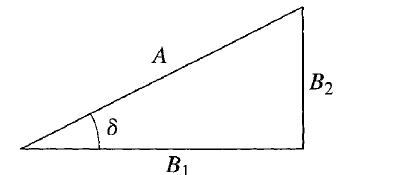
\includegraphics[width=0.3\textwidth]{Triangle.PNG}
			\caption{}
			\label{Triangle}
		\end{figure}
	\item Now we have the cute form
	\begin{align}
	\begin{split}
		x(t) &= A \bigg[\frac{B_1}{A}\cos(\omega t) +  \frac{B_2}{A} \sin(\omega t) \bigg] \\
		&= A \bigg[\cos\delta\cos(\omega t) +  \sin\delta \sin(\omega t) \bigg]  \\
		&= A \cos(\omega t - \delta) 
	\end{split}
	\label{5.11}
	\end{align}
\end{itemize}

\subsubsection{Sln Real Part of Complex Exp}
\begin{itemize}
	\item Rewrite equation~\ref{5.5} by doing the following:
	\begin{align}
		C_1 = \frac{1}{2} (B_1 - i B_2) \quad &and \quad C_2 = \frac{1}{2} (B_1 + i B_2) \\
		C_2 &= C_1^* 
	\end{align}
	\item Now we can write $x$ as the following \footnote{Recall $z + z^* = 2\Re z$}
	\begin{align}
		x(t) &= C_1 \exp^{i\omega t}  + C_1^* \exp^{-i\omega t} \\
		&= 2 \Re[C_1 \exp^{i \omega t}]
	\end{align}
	\item We can even do just a \textit{little} more  related to figure ~\ref{Triangle} to obtain
	\begin{align}
		x(t) = 2 \Re[C_1 \exp^{i \omega t}] = \Re[A \exp^{i (\omega t - \delta)}]
	\end{align}
\end{itemize}

\subsubsection{Energy Considerations}
\begin{itemize}
	\item For the simple case of eq.~\ref{5.11}, the potential $U$ and kinetic energy $T$ are
	\begin{align}
		U &= \frac{1}{2} k A^2 \cos^2(\omega t - \delta)  \\
		T &= \frac{1}{2}m \dot{x} = \frac{1}{2} k A^2 \sin^2(\omega t - \delta)
	\end{align}
	and the total energy is constant (true for any conservative force):
	\begin{equation}
		E = T + U = \frac{1}{2} k A^2 
		\label{5.16}
	\end{equation}
\end{itemize}


\subsection{\green{2D Oscillators}}
\begin{itemize}
	\item Simplest case: \blue{isotropic harmonic oscillator.} Restoring force is direction-independent.
	\begin{itemize}
		\item Restoring force:
			\begin{equation} \bm{F} = -k \bm{r} \label{5.17} \end{equation}.
		\item Technique/steps for analyzing 2D case: First, write force equations in components.
		\begin{align}
		\begin{split}
			\ddot{x} &= \omega^2 x \\
			\ddot{y} &= \omega^2 y
		\end{split}
		\label{5.18}
		\end{align}
		\item We can write these in the same form as eq ~\ref{5.11}, but define the origin of time such that we can dispose of x phase shift $\delta_x$. 
		\begin{align} \tag{5.20}
		\begin{split}
			x(t) &= A_x \cos(\omega t) \\
			y(t) &= A_y \cos(\omega t - \delta)
		\end{split}
		\label{5.20}
		\end{align}
		where $\delta = \delta_y - \delta_x$ is the \blue{relative phase} of the y and x oscillations. 
	\end{itemize}
	\item In the case of \blue{anisotropic oscillator}, we have
	\begin{equation} \tag{5.21}
		F_x = -k_x x \quad F_y = -k_y y \quad F_z = -k_z z 
		\label{5.21}
	\end{equation}
\end{itemize}


\subsection{\green{Damped Oscillations}}
\begin{itemize}
	\item ``\textellipsis resistive forces that will damp the oscillations.''
	\item Assume resistive force is proportional to $v$: $\bm{f} = -b \bm{v}$. 
	\item Consider a cart attached to a spring. 
	\begin{itemize}
		\item Newton's second law:
		\begin{align} \tag{5.24}
			m\ddot{x} + b\dot{x} + kx = 0
			\label{5.24}
		\end{align}
		\item Define the following $\beta$ as the \blue{\textbf{damping constant}}. 
		\begin{align} \tag{5.26}
			\frac{b}{m} = 2 \beta
			\label{5.26}
		\end{align}
		which characterizes strength of damping force. 
		\item Denote $\omega$ as $\omega_0$ now, to distinguish it as the \blue{\textbf{natural frequency}}, freq. it oscillates w/o resistive forces present. $\omega_0 = \sqrt{k/m}$. 
	\item Equation of motion for damped oscillator \mybox[gray!20]{
		\begin{align} \tag{5.28}
			\ddot{x} + 2 \beta \dot{x} + \omega_0^2 x = 0
			\label{5.28}
		\end{align}}
	\end{itemize}
	\newpage
	\item \textbf{Math} to solve the ODE of eqn~\ref{5.28}:
	\begin{itemize}
		\item Let $x(t) = \exp^{rt}$. Plugging in yields the \blue{auxiliary equation} of ~\ref{5.28}.
		\begin{align}
		\tag{5.30}
			r^2 + 2 \beta ~ r + \omega_0^2 = 0
		\label{5.30}
		\end{align}
		\item With the two solutions
		\begin{align}
		\tag{5.31}
		\begin{split}
			r_1 &= - \beta + \sqrt{\beta^2 - \omega_0^2} \\
			r_2 &= - \beta - \sqrt{\beta^2 - \omega_0^2}
		\end{split}
		\label{5.31}
		\end{align}
		\item Thus, we have the general solution of ~\ref{5.28} as \mybox[gray!20]{
			\begin{align} \tag{5.33}
			x(t) = e^{-\beta t} \bigg(C_1 e^{\sqrt{\beta^2 - \omega_0^2}t} + C_2 e^{-\sqrt{\beta^2 - \omega_0^2}t}\bigg)
			\label{5.33}
			\end{align}}
	\end{itemize}
	
	\item If \blue{undamped}, $\beta = 0$. 
	\item \blue{Weak Damping}: $\beta < \omega_0$, sometimes called \textbf{underdamping}.
	\begin{align} \tag{5.36}
		\sqrt{\beta^2 - \omega_0^2} = i \sqrt{\omega_0^2 - \beta^2} = i \omega_1
	\label{5.36}
	\end{align}
	and thus we can reduce $x(t)$ to similar form as ~\ref{5.11}. 
	\begin{align} \tag{5.38}
		x(t) = Ae^{-\beta t} \cos(\omega_1 t - \delta) \label{5.38}
	\end{align}
	\item \blue{Strong Damping}: $\beta > \omega_0$. (\textbf{overdamping}). Rate at which the motion dies out can be charactereized by $\beta - \sqrt{\beta^2 - \omega_0^2}$. Rate of decay \emph{decreases} when $\beta$ is made bigger. 
	
	\item \blue{Critical Damping}: $\beta = \omega_0$. Equation ~\ref{5.33} becomes just 
	\begin{align} \tag{5.42}
		x(t) = e^{-\beta t} 
	\label{5.42}
	\end{align}
	and so we need to find a second independent solution. Turns out it is:
	\begin{align}
	\tag{5.43}
	x(t) = t e^{-\beta t} \label{5.43}
	\end{align}
	and general solution is
	\begin{align}
	\tag{5.44}
	x(t) = C_1 e^{-\beta t} + C_2 t e^{-\beta t}
	\label{5.44}
	\end{align}
\end{itemize}

\newpage
\subsection{\green{Driven Damped Oscillations}}
\begin{itemize}
	\item Denote external driving force by $F(t)$ so now we have
	\begin{align} \tag{5.45}
		m\ddot{x} + b \dot{x} + kx = F(t)
		\label{5.45}
	\end{align}
	and, as before, can let $b/m = 2\beta$ and, also, let $f(t) = F(t)/m$ be force per unit mass. Then \mybox[gray!20]{
		\begin{align} \tag{5.48}
			\ddot{x} + 2\beta \dot{x} + \omega_0^2 x = f(t)
		\label{5.48}
		\end{align}}
	\item Denote $D$ as some linear differential operator. Key point is that, for $Dx = f$, there exist two special solutions for $x$ denoted as $x_p$ and $x_h$ for \textit{particular} and \textit{homogeneous}, where
	\[
		D(x_p + x_h) = Dx_p + Dx_h = f + 0 = f
	\]
\end{itemize}

\subsubsection{Complex solutions for a Sinusoidal Driving Force}
\begin{itemize}
	\item Consider driving force
	\begin{align}
	\tag{5.56}
		f(t) = f_0 \cos(\omega t)
	\label{5.56}
	\end{align}
	where $\omega$ denotes angular frequency of the \textit{driving force}. 
	\item Substitute this in eq~\ref{5.48}, note that $\sin(\omega t)$ is also a solution, 
	\begin{align}
	\tag{5.60}
		\ddot{z} + 2 \beta \dot{z} + \omega_0^2 z = f_0 e^{i\omega t}
	\label{5.60}
	\end{align}
	where $z(t) = x(t) + iy(t)$, x being solution using cosine, y being the sine solution. 
	\item To solve,
	\begin{align}
		z(t) &= C e^{i\omega t} \\ &\text{ then} \\
		(-\omega^2 + 2 i \beta \omega + \omega_0^2)~C e^{i\omega t} &= f_0 e^{i \omega t} \\ &\text{ is solution if} \\
		C &= \frac{f_0}{ \omega_0^2 -\omega^2 + 2 i \beta \omega }
	\end{align}
	\item Let $C = A^{-i\delta}$ before taking $\Re(z)$. Multiply by complex conj. to get amplitude of the oscillations caused by the driving force $f(t)$: \mybox[gray!20]{
		\begin{align} \tag{5.64}
			CC^* = A^2 = \dfrac{f_0^2}{(\omega_0^2 - \omega^2)^2 + 4 \beta^2 \omega^2}
		\label{5.64}
		\end{align}}
	which is biggest when $\omega_0 \approx \omega$. 
	\item Do math to get 
	\begin{align}\tag{5.65}
		\delta = \arctan\bigg(\frac{2 \beta \omega}{\omega_0^2 - \omega^2}\bigg)
		\label{5.65}
	\end{align}
	\item Recall that we are seeking $\Re(z) = x_p(t) = A \cos(\omega t - \delta)$, which is the \emph{particular} solution. 
	\item The \textbf{general solution} is 
	\begin{align}
	\tag{5.67}
		x(t) = A\cos(\omega t - \delta) + C_1 e^{r_1 t} + C_2 e^{r_2 t}
	\label{5.67}
	\end{align}
	where the two extra terms are called \blue{transients} because they both die out exponentially with time.
	\item If we assume weakly damped ($\beta < \omega_0$) then we can write as \mybox[gray!20]{
		\begin{align} \tag{5.68}
			x(t) = A\cos(\omega t - \delta) + A_{tr} e^{-\beta t} \cos(\omega_1 t - \delta_{tr})
		\label{5.68}
		\end{align}}
	where $A_{tr}$ and $\delta_{tr}$ are arbitrary constants determined by the initial conditions. 
	\item \red{Example 5.3}
	\begin{footnotesize}
		\begin{itemize}
			\item Goal: plot $x(t)$ for a driven (weakly) damped oscillator. Parameters given (see mathematica). 
			\item Answers to questions I have along the way:
			\begin{itemize}
				\item \red{Q}: What is $f_0$? \green{A:} It is the amplitude (divided by the oscillator's mass), first seen in equation~\ref{5.56} as $f(t) = f_0 \cos{\omega t}$. \textbf{Learned:} Distinguish between driving amplitude $f_0$ and oscillation amplitude $A$. 
				\item \red{Q}: Where did $A_{tr}$ and $\delta_{tr}$ go? No mention of them here/ignored. They let
				\begin{align}
				\hspace*{-14ex} A_{tr} e^{-\beta t} \cos(\omega_1 t - \delta_{tr}) \stackrel{?}{=}  e^{-\beta t} \big[B_1 \cos(\omega_1 t) + B_2 \sin(\omega_1 t) \big]
				\end{align}
				\green{Ans:} Aha, appears the deltas have been absorbed via the identity (see ~\ref{Triangle}):
				\begin{align}
				\hspace*{-14ex} A_{tr} \cos(\omega_1 t - \delta_{tr}) =  A_{tr} \big[\tfrac{B_1}{A_{tr}} \cos(\omega_1 t) + \tfrac{B_2}{A_{tr}}\sin(\omega_1 t) \big]
				\end{align}
				such that $\tfrac{B_1}{A_{tr}} = \cos(\delta_{tr})$ and $\tfrac{B_2}{A_{tr}}\sin(\delta_{tr})$. However, I'm not sure what happened to the outside factor of $A_{tr}$.
			\end{itemize}
			\item Although the general solutions of $x$ in eq~\ref{5.67} has the transient terms, the first term, $A\cos(\omega t)$ is called an \blue{attractor} because all solutions will eventually converge to just that term, irrespective of initial conditions. There is a \textit{unique} attractor (for a given driving force). 
		\end{itemize}
	\end{footnotesize}
	\item \textit{The amplitude and phase of the attractor depend on the params of the driving force, which is the subject of the next section.}
\end{itemize}

\newpage
\subsection{\green{Resonance}}
\begin{itemize}
	\item Apart from transient motions that we will ignore, a damped\footnote{appears that damped basically means weakly damped} system responds by oscillating at same frequency $\omega$ as driver but with different amplitude $A$:
	\begin{align}
	\tag{5.71}
	\begin{split}
		x(t) &= A \cos(\omega t - \delta) \\
		A^2 &= \dfrac{f_0^2}{(\omega_0^2 - \omega^2)^2 + 4 \beta^2 \omega^2}
	\end{split}
	\label{5.71}
	\end{align}
	\item Discuss here the case when damping constant $\beta$ is very small. 
	\item Although location of $A_{max}$ depends on whether we vary $\omega_0$ or $\omega$, in both cases we want the denominator
	\begin{align}\tag{5.72}
		(\omega_0^2 - \omega^2)^2 + 4 \beta^2 \omega^2
		\label{5.72}
	\end{align}
	to be a minimum. 
	\item Summary of frequencies seen thus far:
	\begin{align}
		\omega_0 &= \sqrt{k/m} = \text{natural/undamped} \\
		\omega_1 &= \sqrt{\omega_0^2 - \beta^2} = \text{damped} \\
		\omega &= \text{driving freq.} \\
		\omega_2 &= \sqrt{\omega_0^2 - 2 \beta^2}  \Leftrightarrow \max_\omega A
	\end{align}
	where it's important to note that (32) is maximum over $\omega$ \emph{with all else fixed}. General maximum is $\omega_0 \approx \omega$ which gives
	\begin{align}
	\tag{5.74}
		A_{max} \approx \frac{f_0}{2 \beta \omega_0}
	\label{5.74}
	\end{align}
\end{itemize}

\subsubsection{The Q Factor}
\begin{itemize}
	\item Decrease $\beta$ $\longrightarrow$ higher and more narrow resonance peak. 
	\item Sharpness of resonance peak, characterized by the \blue{Q factor}, is indicated by the ratio of its FWHM $\approx 2\beta$ to its position $\omega_0$
	\begin{align}\tag{5.77}
		Q = \frac{\omega_0}{2\beta}
	\label{5.77}
	\end{align}
	which can be interpreted as \textit{we want the width $2\beta$ to be very small compared to system's natural frequency $\omega_0$}.
	\item For weakly damped, $\beta << \omega_0$, we can rewrite definition as
	\begin{align}
		Q = \pi \frac{1/\beta}{2\pi/\omega_0} = \pi \frac{\text{decay time}}{\text{period}}
	\end{align}
\end{itemize}


\subsubsection{Phase at Resonance}
\begin{itemize}
	\item Phase difference by which oscillator lags behind driving force:
	\begin{align}\tag{5.79}
		\delta = \arctan\bigg(\frac{2 \beta \omega}{\omega_0^2 - \omega^2}\bigg)
	\label{5.79}
	\end{align}
\end{itemize}

\subsection{\green{Fourier Series (5.7)}}
\begin{itemize}
	\item Any periodic driving force can be built up from sinusoidal forces using Fourier Series. 
	\item If $f(t)$ is any periodic function with period $\tau$ then\footnote{Note: $cos(2n\pi t/\tau) = cos(n \omega t)$} it can be expressed as the sum \mybox[gray!20]{
		\begin{align} 
			f(t) &= \sum_{n=0}^{\infty} \bigg[ a_n \cos(n \omega t) + b_n \sin(n \omega t) \bigg] \tlab{5.82} \\
			a_n &= \frac{2}{\tau} \int_{-\tau/2}^{\tau/2} f(t)  \cos(n \omega t) \mathrm{d}t  \tlab{5.83}\\
			b_n &= \frac{2}{\tau} \int_{-\tau/2}^{\tau/2} f(t)  \sin(n \omega t) \mathrm{d}t   \tlab{5.84} \\
			a_0 &= \frac{1}{\tau} \int_{-\tau/2}^{\tau/2} f(t)  \mathrm{d}t  \tlab{5.85}\\
		\end{align}}
	where $n \ge 1$ for equations~\ref{5.83} and ~\ref{5.84}
\end{itemize}

\subsection{\green{Fourier on Oscillator (5.8)}}
\begin{itemize}
	\item Goal: Solve for motion of an oscillator that is driven by an \textit{arbitrary} driving force.
	\item Equation of motion:
	\begin{align}
		\ddot{x} + 2\beta \dot{x} + \omega_0^2 x = f
	\end{align}
	where $\beta$ is damping constant, $\omega_0$ natural freq, and $f = f(t)$ is any periodic driving force/mass of period $\tau$. 
	\item Rewrite in compact form: $Dx = f$. 
	\item Procedure for finding $x(t)$:
	\begin{enumerate}
		\item Find the Fourier coefficients $f_n$ in the Fourier series for $f(t)$. 
		\item Calculate the values of $A_n$ and $\delta_n$, defined as:
		\begin{align}
			A_n &= \dfrac{f_n}{\sqrt{(\omega_0^2 - n^2\omega^2)^2 + 4 \beta^2 n^2 \omega^2}} \tlab{5.92} \\
			\delta_n &= \arctan\bigg(\frac{2 \beta_n \omega}{\omega_0^2 - n^2 \omega^2}\bigg) \tlab{5.93} 
		\end{align}
		\item Write down $x(t)$ as the following Fourier series:
		\begin{align}
			x(t)  = \sum_{n=0}^{\infty}  A_n \cos(n \omega t - \delta_n)  \tlab{5.94}
		\end{align}
	\end{enumerate}
\end{itemize}

% ==================================================================
%===================================================================
% CHAPTER 6 - Calculus of Variations
% ==================================================================
% ==================================================================
\clearpage
\twocolumn[
\begin{@twocolumnfalse}
\sexin{Calculus of Variations (Ch. 6)}
\end{@twocolumnfalse}]

\p Want an alternative equation of motion that works equally well in any coordinates, and the required alternative is provided by \blue{Lagrange's equations}. 

\subsection{\green{Two Examples (6.1)}}

\p \blue{Shortest path between two points}. The total length of some arbitrary path between points 1 and 2 is 
\begin{align}
L = \int_1^2 ds = \int_{x_1}^{x_2} \sqrt{1 + y'(x)^2} dx \tlab{6.2}
\end{align}
since $ds = \sqrt{dx^2 + dy^2} = \sqrt{1 + y'(x)^2}$. Therefore, the problem is to find $y(x)$ such that eq~\ref{6.2} is a minimum. 

\myspace 
\p \blue{Fermat's Principle}. Required path is the path for which the time of travel of the light is minimum. Note that the refractive index may vary: $n = n(x, y)$. The problem is to find the path $y(x)$ for which the following integral (derivation included) is a minimum. 
\begin{align}
	\int_1^2 dt &= \int_1^2 \frac{ds}{v} = \frac{1}{c} \int_1^2 n ds \\
	&= \frac{1}{c} \int_1^2 n(x, y) ds = \frac{1}{c} \int_{x_1}^{x_2} n(x, y) \sqrt{1 + y'(x)^2} dx \tlab{6.3}
\end{align}
where we don't necessarily need the $1/c$ for the minimization (it's constant). Remember that the speed of light is $v = c/n$ when traversing medium with index of ref. $n$. 

\myspace 
\p Note: When $df/dx = 0$ at a point $x_0$ but we don't know if max, min, or saddle, we say that $x_0$ is a \textbf{stationary point} of the function $f(x)$. Our problem is to find the \textit{paths} that make integrals like eq~\ref{6.2} stationary. 

\Needspace{25\baselineskip}
\subsection{\green{Euler-Lagrange Eq (6.2)}}

\p The variational problem. Have integral of the form \graybox{
	S = \int_{x_1}^{x_2} f\big[	y(x), y'(x), x \big] dx \tlab{6.4}
	}
\p and want path $y(x)$ from pre-specified point $(x_1, y_1)$ to $(x_2, y_2)$. The following derivation will lead us to the Euler-Lagrange equation, which lets us find the path for which eq~\ref{6.4} is stationary. 
\begin{enumerate}
	\item Denote the \textbf{correct solution} as $y = y(x)$. 
	
	\item Write any other (``wrong path'') as 
	\begin{align}
		Y(x) = y(x) + \alpha \eta(x) \tlab{6.8} 
	\end{align}
	where $\eta(x_1) = \eta(x_2) = 0$. Also notice that this approaches the correct solution as $\alpha \rightarrow 0$. 
	
	\item Now $S = S(\alpha)$ where we've defined $\alpha$ such that $S(\alpha = 0)$ is a \textbf{minimum}. 
	\begin{align}
		S(\alpha) &= \int_{x_1}^{x_2} f\big(y + \alpha \eta,~ y' + \alpha \eta', x\big) dx \tlab{6.9}\\
		\pderiv{S}{\alpha} &= \int_{x_1}^{x_2} \bigg( \eta \pderiv{f}{y} + \eta' \pderiv{f}{y'} \bigg) dx = 0 \tlab{6.10}
	\end{align}
	where I'm assuming we can get away with partial derivs being wrt y instead of Y since we are only trying to analyze the case where $\alpha = 0$. 
	
	\item Integrate by parts on the second term, take advantage of boundary condition\footnote{$\eta(x_1) = \eta(x_2) = 0$}, and substitute back in to get
	\begin{align}
		\int_{x_1}^{x_2}  \eta(x) \bigg( \pderiv{f}{y} - \deriv{}{x} \pderiv{f}{y'} \bigg) dx = 0 \tlab{6.12}
	\end{align}
	
	\item Since eq.~\ref{6.12} must be true for all $\eta(x)$ in range $x_1 \le x \le x_2$, we know that \graybox{
		\pderiv{f}{y} - \deriv{}{x} \pderiv{f}{y'}  = 0 \tlab{6.13}
	}
	for all $x_1 \le x \le x_2$. This is the \blue{Euler-Lagrange Equation}. 
\end{enumerate}

\myspace
\p \blue{Procedure: Using EL equation.}
\begin{enumerate}
	\item Set up the problem so that the quantity whose stationary path you seek is expressed in form of eq.~\ref{6.4}. 
	
	\item Write down the EL equation~\ref{6.13}. 
	
	\item Solve this differential equation for the function $y(x)$ that defines the required stationary path. 
\end{enumerate}


\Needspace{20\baselineskip}
\subsection{\green{Applications (6.3)}}

\p \blue{[Ex. 6.1] Shortest Path Between Two Points}. Know that the length of the path is given by ~\ref{6.2}. Notice that we \textit{began} with a quantity in the form of an integral here. We can then simply identify 
\begin{align}
	f(y, y', x) = \big(1 + y'^2\big)^{1/2} \tlab{6.15}
\end{align}
Since 
\begin{align}
\pderiv{f}{y} = 0 \text{ and } \pderiv{f}{y'} = \frac{y'}{\sqrt{1 + y'^2}} \tlab{6.16}
\end{align}
we know that 
\begin{align}
\deriv{}{x}\pderiv{f}{y'} = 0 ~ \rightarrow  ~ \pderiv{f}{y'} = \text{const}
\end{align}
which, after doing algebra, gives us that $y'(x)^2$ is constant as well, i.e. that $y(x) = m x + b$ after integration, yielding the equation for a straight line.\footnote{Note on the total derivative: If $z =  z(x, y)$, then $dz \triangleq \pderiv{z}{x} dx + \pderiv{z}{y} dy$. This can be used to find either $\deriv{z}{x}$ or $\deriv{z}{y}$, for example.}

\myspace
\p \blue{[Ex 6.2] Brachistochrone}. Problem: What shape should we build roller coaster track such that car released from point 1 reaches point 2 in shortest possible time? \myfig{Brach.PNG} 

\p Since $v(y) = \sqrt{2gy}$, take $y$ as the independent variable and write path as $x = x(y)$. Therefore, the time to travel from 1 to 2 is
\begin{align}
t_{12} &= \int_1^2 \frac{ds}{v} \tlab{6.17} \\
&= \frac{1}{\sqrt{2g}} \int_0^{y_2} \dfrac{\sqrt{x'^2 + 1} }{ \sqrt{y} } dy \tlab{6.19}
\end{align}
Again, when we evaluate the derivatives in the EL equation, we end up with $\pderiv{f}{x'}$ as a constant. Let
\begin{align}
\bigg(\pderiv{f}{x'}\bigg)^2 &= \dfrac{x'^2}{y (1 + x'^2)} = const = \frac{1}{2a} \tlab{6.22}
\end{align}
which, after solving for $x'$, we can feed into the following to obtain the path $x(y)$:
\begin{align}
x(y) &= \int x'(y) dy  \\
&= \int \sqrt{\frac{y}{2a - y}} dy \tlab{6.23}
\end{align}
Let $y = a(1 - \cos\theta)$. Then
\begin{align}
x &= a \int (1 - \cos\theta) d\theta \\
&= a(\theta - \sin\theta) + const \tlab{6.25}
\end{align}
and now we have $x(\theta)$ and $y(\theta)$ (parametric equations). 


% ==================================================================
%===================================================================
% CHAPTER 6 - Lagrange's Equations
% ==================================================================
% ==================================================================
\clearpage
\twocolumn[
\begin{@twocolumnfalse}
	\sexin{Lagrange's Equations (Ch. 7)}
\end{@twocolumnfalse}]

\p Advantages over Newtonian formulation:
\begin{enumerate}
	\item Take same form in any coordinate system.
	\item In treating constrained systems, Lagrangian approach eliminates the forces of constraint (like normal force). 
\end{enumerate}

\subsection{\green{Unconstrained Motion (7.1)}}

\p For a particle moving unconstrained in 3D, subject to a conservative net $F(\R)$:
\begin{align}
T &= \onehalf \left( \dot x^2 + \dot y^2 + \dot z^2 \right) \tlab{7.1} \\
U(\R) &= U(x, y, z) \tlab{7.2} \\
\mathcal{L} &= T - U \tlab{7.3} \\
\pderiv{\mathcal{L}}{x} &= - \pderiv{U}{x} = F_x \tlab{7.4} \\
&= \deriv{}{t}\pderiv{\mathcal L}{\dot x} \tlab{7.6} \\
\pderiv{\mathcal L}{\dot x} &= \deriv{T}{\dot x}  = m\dot x = p_x \tlab{7.5} 
\end{align}
where eq~\ref{7.6} implies that 
\begin{quote}
	\blue{[Hamilton's Principle]:} The path followed by a particle between two points 1 and 2 in a given time interval $t_1$ to $t_2$ is such that the action integral, 
	\begin{align}
		S = \int_{t_1}^{t_2} \mathcal L dt \tlab{7.8}
	\end{align} 
	is stationary when taken along the actual path.
\end{quote}

\myspace
\p \blue{Generalized Coordinates} Each position $\bm{r}$ specifies a unique value of $(q_1, q_2, q_3)$ and vice versa\footnote{\textbf{Warning:} `` Although Lagrange's equations are true for any choice of generalized coordinates $q_1, q_2, q_3$ --- and these generalized coordinates may in fact be the coordinates of a noninertial reference frame --- we must be careful that when we first write down the Lagrangian $\mathcal L = T - U$ we do so in an inertial frame.''}
:
\begin{align}
	q_i &= q_i(\bm{r}) \quad \text{for } i=1,2,3 \tlab{7.9} \\
	\bm{r} &= \bm{r}(q_1, q_2, q_3) \tlab{7.10}
\end{align}
which allows us to call the following expressions the \green{generalized force} and \green{generalized momentum}, respectively:
\graybox{
	\pderiv{\mathcal{L}}{q_i} &= \text{(ith component of g.f.)} \tlab{7.15} \\
	\pderiv{\mathcal{L}}{\dot q_i} &= \text{(ith component of g.m.)} \tlab{7.16} \\
	\text{where } \pderiv{\mathcal{L}}{q_i} &= \deriv{}{t} \pderiv{\mathcal{L}}{\dot q_i}
	}

\myspace
\p \purple{[Example 7.2]}. One particle in 2D with Polar Coordinates. 
\begin{itemize}
	\item $\mathcal L(r, \phi, \dot r, \dot{\phi}) = \onehalf m \left( \dot r^2 + r^2 \dot \phi^2 \right) - U(r, \phi)$
	\item \textbf{The r Equation}. 
	\begin{align}
		\pderiv{\mathcal L}{r} &= \deriv{}{t}\pderiv{\mathcal L}{\dot r} \\
		mr\dot{\phi}^2 - \pderiv{U}{r} &= m\ddot r \tlab{7.19} \\
		F_r &= m(\ddot r - r \dot \phi^2) \tlab{7.20}
	\end{align}
	
	\item \textbf{The $\phi$ Equation}. Results in (torque) = (rate of change of angular momentum). 
	\begin{align}
		\pderiv{\mathcal L}{\phi} &= \deriv{}{t}\pderiv{\mathcal L}{\dot \phi} \tlab{7.21} \\
		- \pderiv{U}{\phi} &= \deriv{}{t}( m r^2 \dot \phi) \tlab{7.22} \\
		\nabla U  &= \pderiv{U}{r} \hat{\bm{r}} + \frac{1}{r}\pderiv{U}{\phi}\hat{\bm{\phi}} \tlab{7.23} \\
		\Gamma &= \deriv{L}{t} \tlab{7.24}
	\end{align}
	
\end{itemize}

\subsection{\green{The Plane Pendulum (7.2)}}

\p Consider the simple pendulum shown below. 
\myfig[0.15\textwidth]{PlanePendulum.PNG}

\p The only degree of freedom is the angle $\phi$. The Lagrangian for this pendulum is
\begin{align}
\mathcal L &= \onehalf m l^2 \dot{\phi}^2 - mgl(1 - \cos\phi) \tlab{7.30} 
\end{align}
\textit{Whichever way we proceed, the Lagrangian is written in terms of a single generalized coordinate $q$ and $\dot q$.} This would be true even if we wrote in terms of $x$ and $y$ --- i.e. $\mathcal L$ ``knows'' how many DOF there really are. Luckily, we chose the right (single) coordinate $\phi$. 

\Needspace{14\baselineskip}
\subsection{\green{General Constrained Sys. (7.3)}}

\p \blue{Exact definitions}. Consider arbitrary system of $N$ particles, $\alpha = 1,\ldots,N$ with positions $\bm{r}_\alpha$. The params $q_1,\ldots,q_n$ are a set of \textbf{generalized coordinates} for the system if each 
\begin{align}
\bm{r}_\alpha &= \bm{r}_\alpha(q_1, \ldots, q_n, t) \quad [\alpha = 1,\ldots,N]  \tlab{7.34} \\
q_i &= q_i(\bm{r}_1, \ldots, \bm{r}_N, t) \quad [i = 1,\ldots,n]  \tlab{7.35}
\end{align}
and require that the number of gen. coords $n$ is the \textit{smallest} number that allows the system to be parameterized in this way. In 3D world, $n \le 3N$, and is usually less.

\myspace
\p \blue{Double Pendulum}. In the double pendulum below (\purple(Fig 7.3)), system can be described in terms of four cartesian coordinates (of the bobs) or the generalized coordinates $\phi_1$ and $\phi_2$ shown in the figure.
\myfig[0.15\textwidth]{DoublePendulum.PNG}

\begin{align}
\bm{r}_1 &= \big( l_1 \sin\phi_1, ~ l_1\cos\phi_1  \big) = \bm{r}_1(\phi_1) \tlab{7.37} \\
\begin{split}
\bm{r}_2 &= \big(l_1 \sin\phi_1 + l_2 \sin\phi_2, ~ l_1\cos\phi_1 + l_1\cos\phi_2\big) \\
&= \bm{r}_2(\phi_1, \phi_2) 
\end{split}\tlab{7.38}
\end{align}

This transformation from Cartesian (r) to generalized ($\phi$) coordinates does not depend on time, which defines the generalized coordinates $\phi$ as \green{natural}. 

\myspace
\p \blue{Degrees of Freedom}. Def: the number of coordinates that can be independently varied in a small displacement. For example, a gas of $N$ particles has $3N$ DOF. When the NDOF of an $N$ particle system in 3D is less than 3N, the system is \green{constrained}. If the NDOF is equal to the number of generalized coordinates needed to describe the system's configuration, the system is said to be \green{holonomic}\footnote{Nonholonomic example: a ball rolling on a horizontal table. NDOF=2 but need more than the two naive coordinates $(x, y)$ since the \textit{orientation} of the ball can change (this is extremely annoying because most people would assume the orientation doesn't matter because we are physicists and this is a stupid problem).} We assume all systems hereafter are holonomic, because without this condition, we cannot [guarantee that] Lagrange's equations give the time-evolution of the system. 

\Needspace{14\baselineskip}
\subsection{\green{Proof: L.Eq. W/Constraints (7.4)}}

\p The Lagrangian approach aims to formulate equations \textit{not} involving constraint forces\footnote{Constraint forces examples: (1) wire on a bead -- normal force of bead; (2) particle on a surface -- normal force of surface.}. Assumptions and definitions:
\begin{align}
 \bm{F} &= \nabla U(\bm r, t) \tlab{7.41} \\
 \mathcal L &= T - U \tlab{7.42}
\end{align}
where the total force is $\bm F_{tot} = \bm F_{cstr} + \bm F$. Note that it is the \textit{independence}\footnote{Independent here means each generalized coordinate can be independently varied.} of the generalized coordinates that lets us use the Lagrange equations without worrying about constraints.

\myspace
\Needspace{14\baselineskip}
\subsection{\green{Examples of Lagrange's Eqs (7.5)}}

\p \blue{[7.3] Atwood's Machine}. Goal: solve Lagrange E.O.M for $\ddot x$. 
\myfig[0.12\textwidth]{Atwood.PNG}

\begin{compactitem}
	\item \textbf{Let x be generalized coord.} Reasoning: Notice that heights $x$ and $y$ cannot vary independently. $l = x + \pi R + y$, therefore
	\begin{align}
		y = -x + \text{const.} \tlab{7.53}
	\end{align}
	
	\item \textbf{Write $T$ and $U$.}. Reasoning: Notice that $\dot y = - \dot x$. Therefore\footnote{How to think about potential energy: 
		\begin{compactitem}
			\item Consider each mass by itself.
			\item Consider the work done by gravity should the mass move from its current position to the center of the circle (i.e. a distance -x for $m_1$). 
			\item This work is clearly negative, and equal to -$m_1 g x$ for $m_1$. 
		\end{compactitem}
			} % end footnote
	$$ T = \onehalf (m_1 + m_2) \dot x^2$$
	$$ U = - m_1 g x - m_2 g y = - ( m_1 - m_2 ) g x + \text {const.} $$
	
	
	\item \textbf{Solve for $\ddot x$}. 
	\begin{align}
		\mathcal L &= \onehalf (m_1 + m_2) \dot x^2 + ( m_1 - m_2 ) g x \tlab{7.54} \\
		\pderiv{\mathcal L}{x} = \deriv{}{t}\pderiv{L}{\dot x} &\rightarrow   ( m_1 - m_2 ) g  = (m_1 + m_2) \ddot x \tlab{7.55} \\
		\ddot x &= \dfrac{m_1 - m_2}{m_1 + m_2} g \tlab{7.56}
	\end{align}
\end{compactitem}

\myspace
\p \blue{[7.4] Particle Confined to Cylinder Surface}. Given that only force on the mass is $\bm F = -k \bm r$ (toward origin.)
\myfig[0.15\textwidth]{Cylinder.PNG}

\begin{compactitem}
	\item \textbf{Obtain generalized coordinates}. They are $(z, \phi)$ since $\rho =R$ fixed. 
	\item \textbf{Write $\mathcal L$.} First evaluate velocity component-wise:
	$$v_\rho = 0 \quad v_\phi = R\dot \phi \quad v_z = \dot z$$
	\begin{align}
		\mathcal L = \onehalf m(R^2 \dot{\phi}^2 + \dot z^2) - \onehalf k (R^2 + z^2) \tlab{7.57}
	\end{align}
	
	\item \textbf{Solve Lagrange Eqs for each DOF}. 
	\begin{align}
		-k z &= m \ddot z  \tlab{7.58} \\
		0 &= \deriv{}{t} m R^2 \dot \phi \tlab{7.59}
	\end{align}
	
	\item \textbf{Analyze}. These equations tell us that (1) particle moves along $z = A\cos(\omega t - \delta)$ with S.H.O; and (2) that mass has constant angular velocity $\dot \phi$. 
\end{compactitem}	

\myspace
\p \blue{[7.5] Block Sliding on a Wedge}. Goal: Find time for $m$ to reach bottom of wedge, if released from rest atop the wedge.
\myfig[0.3\textwidth]{BlockWedge.PNG}

\begin{compactitem}
	\item \textbf{Focus on finding $\ddot q_1$} since this is what we need to obtain the answer. 
	\item \textbf{Find $T$}. First in cartesian coordinates. \red{Analyze motion of $M$ and $m$ separately}\footnote{Note, for the small wedge, that 
		$$
		\bm v = (v_x, ~ v_y) = \big( \dot q_2 + \dot q_1 \cos\alpha, \dot q_1 \sin\alpha ~~ \big)
		$$
	}
	\begin{align}
	\begin{split}
		T &= T_M + T_m \\
		&= \onehalf M \dot q_2^2
		+ \onehalf m (\dot q_1^2 + \dot q_2^2 +  2 \dot q_1 \dot q_2 \cos\alpha) 
	\end{split}\tlab{7.60}
	\end{align}
	
	\item \textbf{Find $U$}. Notice that $+\hat y$ is measured \textit{downward} and $y = 0$ at the top of the wedge. Therefore, the block begins with $U = 0$ remember \footnote{that single values of $U$ mean nothing, all that matters are differences} and ends with $U = -mgy= -mgq_1 \sin \alpha $, which means this is the potential energy:
	$$ U = -mgq_1 \sin \alpha $$
	
	
	\item \textbf{Find $\mathcal L$ and solve for $\ddot q_1$ and $\ddot q_2$}. Derivation is same as always, results:
	\begin{align}
		\ddot q_2 &= - \frac{m}{M + m} \ddot q_1 \cos\alpha \tlab{7.66} \\
		\ddot q_1 &= \dfrac{g\sin\alpha}{1 - \frac{m\cos^2\alpha}{M + m}} \tlab{7.67} 
	\end{align}
	which gives us our answer for the time to reach the bottom of the wedge: $t = \sqrt{2l/\ddot q_1}$. 
\end{compactitem}



\myspace
\p \blue{[7.6] Bead on Spinning Wire Hoop}. 
\myfig[0.15\textwidth]{BeadHoop.PNG}

\begin{compactitem}
	\item \textbf{The Lagrangian}. Generalized coordinate is $\theta$. Bead has velocities
	$$ v_{tan} = R\dot{\theta}, \quad v_{norm} = \rho \omega = (R\sin\theta)\omega $$
	which we can use to write
	\begin{align}
	\begin{split}
		\mathcal L &= T - U \\
		&= \onehalf m R^2 (\dot \theta^2 + \omega^2\sin^2\theta) - mgR(1 - \cos\theta) 
	\end{split}\tlab{7.68}
	\end{align}
	
	\item \textbf{Solve the Lagrange Equations}. Result is
	\begin{align}
		\ddot{\theta} = (\omega^2 \cos\theta - g/R)\sin\theta \tlab{7.69}
	\end{align}
	
	\item \textbf{Equilibrium points}. An equilibrium point is any value $\theta$ --- call it $\theta_0$ --- such that if bead is placed at rest ($\dot \theta = 0$) at $\theta = \theta_0$, \textit{then it will remain at rest at $\theta=\theta_0$}. \textbf{This is guaranteed if $\ddot{\theta} = 0$}. 
	
	\begin{quote}
		We conclude that when the hoop is rotating slowly ($\omega^2 < g/R$), there are just two equilibrium positions, at the bottom and top of the hoop, but when it rotates fast enough ($\omega^2 > g/R$), there are two more, symmetrically placed on either side of the bottom.
	\end{quote}
\end{compactitem}



\myspace
\Needspace{14\baselineskip}
\subsection{\green{Lagrange Multipliers (7.10)}}
\p Sometimes, we \textit{are} interested in the constraint forces and thus want a formulation that includes them. Consider system restricted by a \blue{constraint equation} of the form $f(x, y) = const$. The main points in the derivation of Lagrange multipliers are as follows.
\begin{itemize}
	\item \textbf{Perturb the action}. We know by Hamilton's principle that $\delta S = 0$, where the delta is a change in the actual path followed. For a Lagrangian $\mathcal L = \mathcal L (x, \dot x, y, \dot y)$, this is defined as
	\begin{align}
	\delta S = \int \left(\pderiv{\mathcal L}{x}\delta x  + \pderiv{\mathcal L}{\dot x}\delta \dot x + \pderiv{\mathcal L}{y}\delta y  + \pderiv{\mathcal L}{\dot y}\delta \dot y \right) dt \tlab{7.114}
	\end{align}
	
	\item \textbf{Integrate by parts} on the second and fourth terms\footnote{Let u = the partial deriv of L and let dv be $\delta \dot x dt= \delta(dx/dt)dt$ }
	
	\begin{align}
	\delta S 
	= \int \left(\pderiv{\mathcal L}{x}-\deriv{}{t} \pderiv{\mathcal L}{\dot x} \right) \delta x dt
	+ \int \left(\pderiv{\mathcal L}{y}-\deriv{}{t} \pderiv{\mathcal L}{\dot y} \right) \delta y dt\tlab{7.115}
\end{align}

	\item \textbf{Key Idea:} The perturbed path must also satisfy the constraint, which here was stated as f(x, y) = const. for the original path. Therefore, the displacement must leave this unchanged, i.e. that $\delta f = 0$. 
	\begin{align}
		\delta f = \pderiv{f}{x}\delta x + \pderiv{f}{y} \delta y = 0 \tlab{7.116}
	\end{align}
	
	\item \textbf{Final result:} Multiply eq~\ref{7.116} by some $\lambda(t)$. Add this to equation~\ref{7.115}. 
	\graybox{
		\pderiv{\mathcal L}{x} + \lambda \pderiv{f}{x} &= \deriv{}{t} \pderiv{\mathcal L}{\dot x} \tlab{7.118} \\
		\pderiv{\mathcal L}{y} + \lambda \pderiv{f}{y}&= \deriv{}{t} \pderiv{\mathcal L}{\dot y} \tlab{7.119} \\
		f(x, y) &= \text{const} \tlab{7.120}
		}
\end{itemize} 


\myspace
\p \blue{[Ex 7.8] Atwood's Machine Using Lagrange Multiplier}. 



% ==================================================================
%===================================================================
% CHAPTER 8 - TWO-BODY PROBLEMS
% ==================================================================
% ==================================================================
\clearpage
\twocolumn[
\begin{@twocolumnfalse}
	\sexin{Two-Body Problems (Ch. 8)}
\end{@twocolumnfalse}]

\subsection{\green{The Problem}}
\begin{itemize}
	\item Two points particles where only forces of interest are $\F_{12}$ and $\F_{21}$ their mutual conservative/central interaction.
	\item The forces can be derived from a potential\footnote{A conservative force is dependent only on the position of the object. If a force is conservative, it is possible to assign a numerical value for the potential at any point. When an object moves from one location to another, the force changes the potential energy of the object by an amount that does not depend on the path taken.} energy $U(\R_1, \R_2)$. 
	\item If a conservative force is central, then $U$ is independent of the \underline{direction} of $(\R_1 - \R_2)$ (only depends on the magnitude). 
	\item Denote $\R = \R_1 - \R_2$ as the \blue{relative position} of body 1 to body 2. 
\end{itemize}

\subsection{\green{Rel. Coords/Reduced Mass}}
\begin{itemize}
	\item Want generalized coordinates to solve problem. Recall that the \blue{center of mass position} $\bm{R}$ of the two bodies is
	\begin{align}\tag{8.7}
		\bm{R} = \dfrac{m_1 \R_1 + m_2 \R_2}{M}
		\label{8.7}
	\end{align}
	which lies along the line joining the two bodies. 
	\item Total momentum of the two bodies is $\bm{P} = M \dot{\bm{R}}$, which is constant $\rightarrow \dot{\bm{R}}$ is constant $\rightarrow$ we can choose the \blue{CM frame} in which the CM is at rest. 
	\item Want to find the kinetic energy in generalized coord system of $\R$ and $\bm{R}$. Recall that 
	\begin{align}
		\R_1 &= \bm{R} + \frac{m_2}{M}\R \\
		\R_2 &= \bm{R} - \frac{m_1}{M}\R 
	\end{align}
	which leads to 
	\begin{align}
		T &= \onehalf \bigg( m_1 \dot{\R_1}^2 + m_2 \dot{\R_2}^2 \bigg) \\
		&= \onehalf \bigg( M\dot{\bm{R}}^2 + \mu \dot{\R}^2 \bigg) 
	\end{align}
	where $\mu$ is the \blue{reduced mass}, defined as \mybox[gray!20]{
		\begin{align} \tag{8.11}
			\mu = \dfrac{m_1 m_2}{M}
		\label{8.11}
		\end{align}}
\end{itemize}

\newpage
\subsection{\green{Equations of Motion}}
\begin{itemize}
	\item Lagrange equations for $\bm{R}$ and $\R$ respectively:
	\begin{align} 
		\dot{\bm{R}} &= \text{const}  	\tag{8.14}\label{8.14} \\
		\mu \ddot{\R} &= - \nabla U(\R) \tag{8.15}\label{8.15}
	\end{align}
	and thus, to solve for the relative motion, we have only to solve Newton's second law for a single particle of mass $\mu$ and position $\R$, with potential energy $U(r)$. 
\end{itemize}

\subsubsection{The CM Frame}
\begin{itemize}
	\item Due to eq~\ref{8.14}, we can choose the \blue{CM-frame}, in which the CM is at rest and the total momentum is zero. 
\end{itemize}

\subsubsection{Conservation of Angular Momentum}
\begin{itemize}
	\item The angular momentum in the CM frame is
	\begin{align}\tag{8.19}
	\begin{split}
		\bm{L} &= \frac{m_1m_2}{M}\bigg(m_2 \R \times \dot{\R} + m_1 \R \times \dot{r} \bigg) \\
		&= \R \times \mu \dot{\R}
	\end{split}
	\label{8.19}
	\end{align}
	which is \textit{constant} since angular momentum conserved. 
	\item In CM frame, whole motion remains in a fixed plane.
\end{itemize}

\subsubsection{The Two Equations of Motion}
\begin{itemize}
	\item Do Lagrangian stuff to get equations of motion:
	\begin{align}
	\mu r^2 \dot{\phi} = \text{const} &= \ell \\
	\mu r \dot{\phi}^2 - \deriv{U}{r} &= \mu \ddot{r}
	\end{align}
	the $\phi$ and $r$ equations, respectively. 
\end{itemize}

\newpage
\subsection{\green{Equivalent 1D Problem (8.4)}}
\begin{itemize}
	\item Since $\dot{\phi} = \ell/\mu r^2$, we can rewrite
	\begin{align}
		\mu\ddot{r} = -\deriv{U}{r} + \mu r \dot{\phi}^2 = -\deriv{U}{r} + F_{cf}
	\end{align}
	so the particle's radial motion is same as if particle were subject to actual force $-\deriv{U}{r}$ plus a centrifugal force. 
	\item Can use math to express $F_{cf}$ as gradient of some $U_{cf}$. 
	\begin{align}
		F_{cf} &= -\deriv{}{r} \bigg(\frac{\ell^2}{2\mu r^2}\bigg) \\
		&= -\deriv{U_{cf}}{r}
	\end{align}
	\item Now, we can rewrite radial equation with an \blue{effective potential}, defined as the sum of $U$ and $U_{cf}$. \mybox[gray!20]{
		\begin{align} \tag{8.29}
			\mu \ddot{r} &= - \deriv{}{r} \big[ U(r) + U_{cf}(r) \big] = - \deriv{}{r}U_{eff}(r) \label{8.29} \\
			U_{eff}(r) &= U(r) + U_{cf}(r) = U(r) + \frac{\ell}{2\mu r^2} \label{8.30}\tag{8.30}
		\end{align}}
\end{itemize}

\subsubsection{Conservation of Energy}
\begin{itemize}
	\item Multiply both sides of eq~\ref{8.29} and move terms to LHS to get
	\begin{align}
		\onehalf \mu \dot{r}^2 + U_{eff}(r) &= \text{const} 				\tlab{8.34} \\
		\onehalf \mu \dot{r}^2  + \onehalf \mu r^2 \dot{\phi}^2 + U(r) &= E \tlab{8.35}
	\end{align}
	which is conservation of energy. 
\end{itemize}
%
% _________________________ SECTION 8.5 ______________________________
% 
\subsection{\green{Equation of Orbit (8.5)}}
\begin{itemize}
	\item Eq~\ref{8.29} gives $r(t)$. Now we seek $r(\phi)$. Tells us about shape of the orbit. 
	\item Main parts of derivation from $r(t) \rightarrow u(\phi)$:
	\begin{align}
		\mu \rddot &= F(r) + \frac{\ell^2}{\mu r^3} && \footnotesize{\text{Radial equation}} \tlab{8.37} \\
		u &= \frac{1}{r} && \footnotesize{\text{Define substitution}} \tlab{8.38} \\
		\ddt{} &= \frac{\ell u^2}{\mu} \ddphi{} &&  \footnotesize{\text{Chain rule on }\phi} \tlab{8.39} \\
		%&= &&  \footnotesize{\text{}} \tlab{8.} \\
	\end{align}
	which, after applying to the radial equation and shifting some terms around yields \mybox[gray!20]{
	\begin{align}
		u''(\phi) &= -u(\phi) - \frac{\mu}{\ell^2 u(\phi)^2}F \tlab{8.41}
	\end{align}}
	\item If we solve eq~\ref{8.41}, we have $r(\phi) = 1/u(\phi)$. 
	\item \blue{Example 8.3: Radial Equation for a Free Particle:}
	\begin{footnotesize}
	\begin{itemize}
		\item If no external forces, expect ``orbit'' to be straight line. 
		\item Transformed radial equation is 
		\begin{equation}
			u''(\phi) = -u(\phi) \rightarrow u(\phi) = A\cos(\phi-\delta) \tlab{8.42}
		\end{equation}
		\item Which means we can write $r(\phi) = \tfrac{r_0}{\cos(\phi-\delta)}$, the equation for a line in polar coordinates.
	\end{itemize}
	\end{footnotesize}
\end{itemize}
%
% _________________________ SECTION 8.6 ______________________________
% 
\subsection{\green{The Kepler Orbits (8.6)}}
\begin{itemize}
	\item The \blue{Kepler Problem}: Find the possible orbits of any object subject to an inverse-square force. 
	\item Write general inverse-square force as
	\begin{align}
		F(r) = -\frac{\gamma}{r^2} = -\gamma u^2 \tlab{8.44} 
	\end{align}
	\item Main parts of deriving $r(\phi)$ for inverse-square force:
	\begin{align}
	u''(\phi) &= -u(\phi) + \gamma\mu/\ell^2 &&  \footnotesize{\text{Plug in to radial eq.}} \tlab{8.45} \\
	u(\phi) &= \frac{\gamma\mu}{\ell^2} + A\cos\phi &&  \footnotesize{\text{General solution}} \tlab{8.47} \\
	r(\phi) &= \dfrac{c}{1 + \epsilon\cos\phi} &&  \footnotesize{\text{Solve for r}} \tlab{8.49} \\
	%&= &&  \footnotesize{\text{}} \tlab{8.} \\
	\end{align}
	where we've defined constants\footnote{$c$ has the dimensions of length. $\epsilon$ is assumed positive} $c = \ell^2/\gamma\mu$ and $\epsilon = A\ell^2/\gamma\mu = Ac$. 
	\item Recap: This is the (very) general solution of $r(\phi)$ in the case of some inverse-square (central) force. 
\end{itemize}

\subsubsection{The Bounded Orbits}
\begin{itemize}
	\item $\epsilon=1$ is boundary between \textbf{bounded} ($\epsilon<1$) and unbounded ($\epsilon\ge 1$) orbits.\footnote{Again, $\epsilon$ is ALWAYS assumed $\epsilon > 0$.}
	\item With $\epsilon<1$, $r$ oscillates between\footnote{Note that ratio of $r$ max/min can be determined give $\epsilon$}
	\begin{align}
		r_{min} &= \frac{c}{1+\epsilon} &&  \footnotesize{\text{\red{PERIHELION}}} \tlab{8.50A} \\
		r_{max} &= \frac{c}{1-\epsilon} &&  \footnotesize{\text{\red{APHELION}}} \tlab{8.50B} 
	\end{align}
	\item Since $r(0) = r(2\pi)$, orbit closes on itself after one revolution.
	\item Orbit is an ellipse. Can rewrite eq~\ref{8.49} as \begin{scriptsize}
		\begin{align}
			\tfrac{(x+d)^2}{a^2} + \frac{y^2}{b^2} = 1 \text{ where } a = c/(1-\epsilon^2);b=c/\sqrt{1-\epsilon^2};d=a\epsilon
		\end{align}
	\end{scriptsize}
	\item We can now identify $\epsilon$ as the \blue{eccentricity of the ellipse}.
	\begin{align}
		\frac{b}{a} = \sqrt{1 - \epsilon^2} \tlab{8.53}
	\end{align}
	where (1) $\epsilon=0=\text{circle}$, (2) $\epsilon\rightarrow 1=\text{parabola}$, and (3) $\epsilon>1=\text{hyperbola}$.
	\begin{figure}[t]
		\centering
		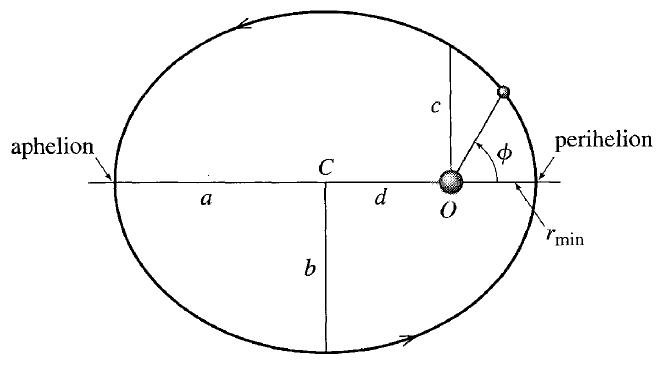
\includegraphics[width=0.3\textwidth]{EllipseOrbit.PNG}
		\caption{Center at $x=-d$. Sun at one foci at origin.}
		\label{fig:8.10}
	\end{figure}
	\item Now we have \blue{Kepler's first law} (see figure~\ref{fig:8.10}):
	 \begin{quote}
		The planets follow orbits that are ellipses with the sun at one focus.
	\end{quote}
\end{itemize}

\subsubsection{Orbital Period; 3rd Law}
\begin{itemize}
	\item \begin{small}See page 312 for more details. Helpful info on ellipses/kepler. Don't want to copy everything here.\end{small}
	\item Resul: for all bodies orbiting the sun, square of period $\propto$ cube of semimajor axis. \mybox[gray!20]{
		\begin{align}
		\tau^2 = \dfrac{4\pi^2}{GM_s} a^3 \tlab{8.55}
		\end{align}}
\end{itemize}

\subsubsection{Relationship: $E$ and $\epsilon$}
\begin{itemize}
	\item Relate eccentricity of orbit to energy of the orbiting body (e.g. planet). 
	\item Energy is equal to the \textit{effective} potential energy when $r = r_{min}$. 
	\begin{align}
		E = U_{eff}(r_{min}) = \frac{\gamma^2 \mu}{2\ell^2}\big(\epsilon^2 - 1 \big) \tlab{8.58}
	\end{align}
	which is true for \textbf{both} bounded and unbounded orbits. 
	\item Note that, for a given value of $\ell$, orbit of lowest possible $E$ is circular orbit with $\epsilon = 0$. 
\end{itemize}

% ==================================================================
%===================================================================
% CHAPTER 9 - NONINERTIAL FRAMES
% ==================================================================
% ==================================================================
\clearpage
\twocolumn[
\begin{@twocolumnfalse}
	\sexin{Mechanics in Noninertial Frames (Ch. 9)}
\end{@twocolumnfalse}]

\subsection{\green{Acceleration (9.1)}}
\p Modified version of Newton's second law in a reference frame $\s$ moving with speed $V$ and acceleration $A = \dot{V}$ relative to some inertial frame $\s_0$:
\graybox{m\rddot &= \F - m\bm{A} = \F - \F_{inertial} \tlab{9.4} \\ 
	\F_{inertial} &= -m\bm{A} \tlab{9.5} }
\p where $\F = m\rddot_0$ is the net force on the ball as seen in (the inertial frame) $\s_0$. 
\myspace

\subsection{\green{The Tides (9.2)}}

\p Caused by gravitational attraction of the moon\footnote{and the sun a little bit.}. 
\myfig{Tides.PNG}

\p Can obtain the \blue{tidal force} by using eq~\ref{9.4}. 
\begin{itemize}
	\item Forces on a mass $m$ near surface of Earth:
	\begin{enumerate}
		\item Earth gravity $m\bm{g}$. 
		\item Moon gravity $-GM_{moon} ~ m \bm{\hat{d}} / d^2$.\footnote{$d$ points from object to center of moon.}
		\item Net other/non-gravity $\F_{ng}$
	\end{enumerate}
	\item Centripetal acceleration of Earth due to moon\footnote{$d_0$ points from earth center to moon center.} is $\bm{A} = -G M_{moon} \bm{\hat{d}_0} / d_0^2$.
	\item Plugging into equation~\ref{9.4} yields
	\graybox{  m\rddot &= m\bm{g} + \F_{tid} -  \F_{ng}  \tlab{9.11} \\ 
		\F_{tid} &= - G M_{moon} ~ m \bigg(\frac{\bm{\hat{d}}}{d^2}  - \frac{\bm{\hat{d}}_0}{d_0^2} \bigg)\tlab{9.12}   }
\end{itemize}
\myspace 

\Needspace{14\baselineskip}
\subsection{\green{Angular Velocity Vector (9.3)}}

\p In discussing \textit{rotation of a rigid body}, only the following two situations concern us (for now):
\begin{enumerate}
	\item Body rotating about a \textit{fixed} point (in some inertial frame). e.g. a wheel spinning about a fixed axle. 
	\item If no fixed point (e.g. baseball spinning as it flies through air), then proceed by 
	\begin{itemize}
		\item Find motion of the CM $\bm{R}(t)$. 
		\item Analyze rotational motion of body relative to its CM via $\R(t)$. 
	\end{itemize}
\end{enumerate}

\p \blue{Euler's Theorem}: \begin{small}\textit{The most general motion of any body relative to a fixed point $O$ is a rotation about some axis through $O$.} \\ \end{small}

\p Denote direction of axis of rotation with $\bm{u}$. Combine with the rate of rotation $\omega$ to get the \blue{angular velocity vector}
\begin{align}
\bm{\omega} = \omega \bm{u} \tlab{9.21}
\end{align}
where the relationship between the angular velocity $\bm{\omega}$ and the linear velocity $\bm{v}$ is 
\graybox{\bm{v} = \bm{\omega} \times \R   \tlab{9.22}}
\myfig{VelocityVector.PNG}
\p and if $\bm{e}$ is \textit{any} vector fixed in the rotating body, then its rate of change as seen from the non-rotating frame is 
\begin{align}
	\deriv{\bm{e}}{t} = \bm{\omega} \times \bm{e} \tlab{9.23} 
\end{align}

\p Finally, note that addition of \emph{relative} velocities is the same for angular and linear.
\begin{align}
	\bm{v}_{31} &= \bm{v}_{32} + \bm{v}_{21} \tlab{9.24} \\
	\bm{\omega}_{31} &= \bm{\omega}_{32} + \bm{\omega}_{21} \tlab{9.25}
\end{align}

% _________________ 9.4 ________________________

\Needspace{14\baselineskip}
\subsection{\green{TimeDeriv Rotating Frame (9.4)}}

\p Consider an arbitrary vector $\bm{Q}$. The time rate of change of $\bm{Q}$ as measured in $\s_0$ in terms of its corresponding rate in $\s$ is
\graybox{ \bigg(\deriv{\bm{Q}}{t}\bigg)_{\s_0} =   \bigg(\deriv{\bm{Q}}{t}\bigg)_{\s}  + \bm{\Omega} \times \bm{Q}   \tlab{9.30}  }
where $\bm{\Omega}$ denotes the (usually known) angular velocity of a noninertial frame $\s$ (relative to $\s_0$). 
\myspace

\subsection{\green{2nd Law in Rot. Frame (9.5)}}

\p Assuming now that $\bm{\Omega}$ is constant. Find that the form of Newton's second law for the rotating frame $\s$ is
\graybox{ m\rddot &= \F + \F_{cor} + \F_{cf} \tlab{9.34/37s} \\
	   F_{cor} &= 2m\rdot \times \bm{\Omega}  \tlab{9.35} \\  
	F_{cf} &= m \big( \bm{\Omega} \times \R \big) \times \bm{\Omega} \tlab{9.36}  }

\p and we have the \blue{coriolis force and centrifugal force}. The takeaway here is that we can use Newton's second law in rotating (and hence noninertial) reference frames, provided we remember to always add these two ``fictitious'' forces. 
\myspace

\subsection{\green{Centrifugal Force (9.6)}}

\p The Coriolis force, which is proportional to object's velocity $\bm{v} = \rdot$, is \textbf{zero} for any object that is at rest in the rotating frame and negligible if moving sufficiently slowly. \textbf{For the rest of the chapter, main concern is rotating frame of the earth}. In this case, 
\begin{align}
	\frac{F_{cor}}{F_{cf}} \sim \frac{v}{R \Omega} \sim \frac{v}{V} \tlab{9.38}
\end{align}
where $v$ is the object's speed relative to the rotating frame of the earth, $R = R_{earth}$, and $V \approx 1000~mi/h$ is the speed of a point on the equator as the earth rotates with angular velocity $\Omega$. Therefore, for objects with $v << 1000~mi/h$, a good approx. is to ignore $\F_{cor}$, which is what we will do in this section. \\

\p Note: The angle $\theta$ in the fig below eq~\ref{9.22} is called the \blue{colatitude}. Also $\F_{cf}$ points radially outward from axis of rotation in the direction of $\hat{\rho}$, thus
\begin{align}
	F_{cf} = m \Omega^2 \rho \hat{\bm{\rho}} \tlab{9.40}
\end{align}

\Needspace{14\baselineskip}
\subsubsection{Free-Fall Acceleration}

\p Denote the familiar $\bm{g}$ now as just $\bm{g}_0$, the \textit{initial} acceleration\footnote{What this means: Immediately after being released \emph{from rest} (and so zero velocity) the Coriolis force is zero. This will change when the object speeds up. Therefore, from here on out, $\bm{g}_0$ is the acceleration solely due to the familiar $-GMm/r^2 = m\bm{g}_0$ force, while $\bm{g}$ is defined in equation~\ref{9.44}.}, relative to earth. The equation of motion is
\begin{align}
	m\rddot &= \F_{grav} + \F_{cf} \equiv \F_{eff} \tlab{9.41} \\
	&= m\bm{g}_0 + m\Omega^2 R \sin\theta \hat{\bm{\rho}} \tlab{9.43} \\
	\bm{g} &= \bm{g}_0 + \Omega^2 R \sin\theta \hat{\bm{\rho}} \tlab{9.44}  \\
	g_{rad} &= g_0 - \Omega^2 R \sin^2\theta \tlab{9.45} \\
	g_{tang} &= \Omega^2 R \sin\theta\cos\theta \tlab{9.47} 
\end{align}
\myfig{FreeFall.PNG}
\myspace 

\subsection{\green{Coriolis Force (9.7)}}

\p When an object is moving, there is a second inertial force that you must include when want to use 2nd law in rotating frame:
\begin{align}
\F_{cor} &= 2m\rdot \times \bm{\Omega} = 2m\bm{v} \times \bm{\Omega}  \tlab{9.49} 
\end{align}
where $\bm{v} = \rdot$ is object's velocity relative to the rotating frame. 
\myfig{Coriolis.PNG}

\p Notice how, in fig above, $F_{cor}$ seems to deflect object's velocity to the right. 

% ___________________ 9.8 FREE FALL AND CORIOLIS FORCE ___________________________
\Needspace{14\baselineskip}
\subsection{\green{Coriolis Free-Fall (9.8)}} 

\p Consider freely falling object close to a point $\bm{R}$ on earth's surface. Equation of motion is 
\begin{align}
	m\rddot = m\bm{g}_0 + \F_{cf} + \F_{cor} \tlab{9.50}
\end{align}
but since $\R$, the position of object relative to center of Earth is $\approx \bm{R}$, we can replace $\F_{cf} \approx m \big(\bm{\Omega} \times \bm{R} \big) \times \bm{\Omega}$. Substituting this in and recalling formula~\ref{9.44} for $\bm{g}$, we can rewrite eq~\ref{9.50} as
\begin{align}
	\rddot = \bm{g} + 2\rdot \times \bm{\Omega} \tlab{9.51}
\end{align}
which doesn't involve the position $\R$ directly at all. Therefore, choose origin at position $\bm{R}$ shown below to make life easier.
\myfig{NewR.PNG}

\p Now, can break into components and solve.
\begin{align}
	\rdot 				&= (\dot{x}, \dot{y}, \dot{z}) \\
	\bm{\Omega} 		&= (0, \Omega\sin\theta, \Omega\cos\theta) \\
	\rdot \times\Omega 	&= \bigg( 	\dot{y}\Omega\cos\theta -  \dot{z}\Omega\sin\theta, ~~
									-\dot{x}\Omega\cos\theta, ~~ 
									\dot{x}\Omega\sin\theta   \bigg) \tlab{9.52}
\end{align}
and the equation of motion, eq~\ref{9.51}, resolves into
\begin{align}
\begin{split}
	\ddot{x} &= 2\Omega(\dot{y}\cos\theta - \dot{z}\sin\theta ) \\
	\ddot{y} &= -2\Omega\dot{x}\cos\theta  \\
	\ddot{z} &= -g + 2\Omega\dot{x}\sin\theta 
\end{split}
\tlab{9.53}
\end{align}

\p \blue{Zeroth-order approximation.} If we ignore $\Omega$ entirely, since it is really small, we get
\begin{align}
x = 0, \quad y = 0, \quad \text{and} \quad z = h - \onehalf g t^2 \tlab{9.55}
\end{align}

\p \blue{First-order approximation.} Since there are no rules in math (amirite?) just plug in eq~\ref{9.55} into eq~\ref{9.53} and solve for x (y and z are the same as zeroth order) to get
\begin{align}
	x = \frac{1}{3} \Omega g t^3 \sin\theta \tlab{9.57}
\end{align}
and if we are bored, can repeat this to get the second-order approximations and so on. Equation~\ref{9.57} tells us that \textbf{a freely falling object does not fall straight down}, due to the Coriolis force. 


% ==================================================================
%===================================================================
% CHAPTER 10 
% ==================================================================
% ==================================================================
\clearpage
\twocolumn[
\begin{@twocolumnfalse}
	\sexin{Rotational Motion of Rigid Bodies (Ch. 10)}
\end{@twocolumnfalse}]


\subsection{\green{Properties of CM (10.1)}}

\graybox{
	\mathbf F &= M \mathbf{\ddot R}	 \tlab{10.3} \\
	\mathbf L &= \mathbf R \times \mathbf P 
				+ \sum_\alpha \bm{r}'_\alpha \times m_\alpha \bm{\dot r}'_\alpha \tlab{10.8} \\
	T &= \onehalf M \mathbf{\dot R}^2 + \onehalf \sum_{\alpha} m_\alpha \bm{\dot r}_\alpha^{\prime 2} \tlab{10.15} \\
	U &= U^{ext} + U^{int} \tlab{10.19}
	}
	
\myspace
\subsection{\green{Rot. about Fixed Axis (10.2)}}

\p Consider rigid body rotating about z axis, and with the origin $O$ somewhere on axis of rotation. The z-component of the angular momentum is given by
\begin{align}
L_z &= \sum m_\alpha (x_\alpha^2 + y_\alpha^2) \omega  \tlab{10.23} \\
&= \sum m_\alpha \rho_\alpha^2 \omega = I_z \omega \tlab{10.24} \\
T &= \onehalf \sum m_\alpha \rho_\alpha^2 \omega^2 = \onehalf I_z \omega^2 \tlab{10.26}
\end{align}
where $I_z$ is the \blue{moment of inertia} about the z-axis. 

\myspace 
\p \blue{Directions of $\mathbf{L}$ and $\bm{\omega}$}. Fig below shows how direction of $L$ and $\omega$ may not coincide. Accordingly, we redefine notation for $L$ and $I$ shown below the figure.
\myfig[0.2\textwidth]{MomInert.PNG}

\p where the two coefficients $I_{xz}$ and $I_{yz}$ are called the \textbf{product of inertia} of the body. 

\myspace\Needspace{10\baselineskip}
\subsection{\green{Inertia Tensor (10.3)}}

\p \textbf{General case}. 
\graybox{
	\mathbf{L} &= \mathbf{I} \bm{\omega} \quad \text{where} \tlab{10.42} \\
	\mathbf{I} &= 
	\begin{bmatrix}
		I_{xx} & I_{xy} & I_{xz} \\
		I_{yx} & I_{yy} & I_{yz} \\
		I_{zx} & I_{zy} & I_{zz} 
	\end{bmatrix}\\
	I_{xx} &= \sum m_\alpha  ( y_\alpha^2 + z_\alpha^2)  \tlab{10.37} \\
	I_{xy} &= -\sum m_\alpha x_\alpha y_\alpha 	\tlab{10.38}
}
and we note that $\mathbf{I}$ is \textbf{symmetric}. 

\myspace
\subsection{\green{Principal Axes of Inertia (10.4)}}

\p A \blue{principal axis} is one where $\mathbf{L}$ and $\bm \omega$ are parallel. Mathematically: any axis with property that if $\bm \omega$ points along it, that 
\begin{align}
\mathbf{L} = \lambda \bm \omega \tlab{10.65}
\end{align}
where $\lambda$ is the \textit{moment of inertia about the axis}. More generally, if $\mathbf I$ is diagonal wrt a chosen set of axes, 
\begin{align}
\mathbf I = 
	\begin{bmatrix}
		\lambda_1 & 0 & 0 \\
		0 & \lambda_2 & 0 \\
		0 & 0 & \lambda_3 
	\end{bmatrix}
\end{align}
then the $\lambda_i$ are called the \blue{principal moments}, the moments of inertia about the 3 principal axes. \emph{Any} rigid body rotating about any point has 3 principal axes. 


\myspace \p \blue{Kinetic Energy}. In general, 
\begin{align}
T = \onehalf \omega \cdot \mathbf L \tlab{10.67}
\end{align}

\myspace
\Needspace{10\baselineskip}
\subsection{\green{Finding Princ. Axes \& Eigval. Eqs (10.5)}}

\p \blue{Procedure}. First, find eigenvalues and then plug in each separately to find eigenvectors. 
\begin{align}
	(\mathbf{I} - \lambda) \omega &= 0 \tlab{10.70} \\
	\det(\mathbf I - \lambda) &= 0 \tlab{10.71} 
\end{align}
Note that this entire process is equivalent to diagonalizing the inertia tensor $\mathbf I$. 

\myspace
\subsection{\green{Top Precession due to Weak Torque (10.6)}}

\p \red{Important:} If a body has two perpendicular planes of reflection symmetry through $O$, then the 3 perpendicular axes defined by these two planes and $O$ are principal axes. Because of the top's axial symmetric, inertia tensor is diagonal. 


\myfig[0.25\textwidth]{SpinningTop.PNG}

\p In the absence of gravity, \purple{$\mathbf{L} = \lambda_3 \omega \bm{e}_3$}, which is constant since no torque. \textit{With} gravity, there is a torque, 
\begin{align}
\bm\Gamma = \mathbf{R}\times M\bm{g} \\ 
| \bm\Gamma | = RMg\sin\theta
\end{align}
and let's assume it is \textit{small}, meaning that although $\bm\Gamma=\dot{\mathbf{L}}$, we can assume the newly nonzero $\omega_1$, $\omega_2$ remain negligibly small compared to $\omega_3$. Then  $\dot{\mathbf{L}}=\bm\Gamma$ becomes
\begin{align}
	\lambda_3 \omega \dot{\bm{e}_3} &=  \mathbf{R}\times M\bm{g}
\end{align}

\myspace
\subsection{\green{Problem-Solving Tips}}

\p \blue{Potential Energy}. 
\begin{compactitem}
	\item The (grav) potential energy of a system is equal to the potential of the CM. 
\end{compactitem}

\myspace
\p \blue{Kinetic Energy}. 
\begin{compactitem}
	\item For a rigid body, the only possible motion rel. to the CM is rotation, therefore
	\begin{align}
		T = \onehalf M \dot{\mathbf R}^2 + \onehalf \sum m_\alpha \dot{\bm r}_\alpha^{\prime 2}
	\end{align}
	
	\item Don't assume kinetic energy is conserved in collisions, since may be inelastic. 
\end{compactitem}

\myspace
\p \blue{Angular momentum}. 
\begin{compactitem}
	\item $\mathbf L$ is conserved \textit{component-wise}, so don't get tripped up about whether or not some component of $L$ is nonzero (e.g. in 10.16). Just focus on conserving the relevant components for the problem. 
\end{compactitem}


\subsection{10.7 - 10. Rapid Summary}

\subsubsection{Euler's Equations}

\p \blue{Frames}. The \textbf{space frame} is any inertial frame (fixed in space), whose axes we label x, y, z. The \textbf{body frame} is the rotating frame, fixed w.r.t. the body, denoted with axis vectors $e_1, e_2, e_3$. In the body frame, angular momentum will be
\begin{align}
\mathbf L &= (\lambda_1\omega_1, \lambda_2\omega_2, \lambda_3\omega_3) \quad \mred{[BODY FRAME]} \tlab{10.84}
\end{align}

\myspace
\p \blue{Euler's Equations} determine the motion of a spinning body as seen in the body frame. Their derivation is sketched below, with the final result in gray.
\begin{align}
\left( \deriv{\mathbf L}{t} \right)_{space}  &= \Gamma	\tlab{10.85}\\
&= \left( \deriv{\mathbf L}{t} \right)_{body}  + \bm{\omega} \times \mathbf L \tlab{10.86}
\end{align}

\graybox{
	\dot{\mathbf L} + \bm{\omega} \times \mathbf L &= \Gamma \quad \mred{[EULER'S~EQ]} \tlab{10.87} \\
	\begin{split}
		\lambda_1\dot{\omega_1} 	- 	(\lambda_2 - \lambda_3) \omega_2\omega_3 &= \Gamma_1 \\
		\lambda_2\dot{\omega_2} 	- 	(\lambda_3 - \lambda_1) \omega_3\omega_1 &= \Gamma_2 \\
		\lambda_3\dot{\omega_3} 	- 	(\lambda_1 - \lambda_2) \omega_1\omega_2 &= \Gamma_3 
	\end{split}\tlab{10.87}
}

\subsubsection{With Zero Torque}

\subsubsection{Euler Angles}

\graybox{
	\omega &= (-\dot{\phi} \sin\theta)e_1' + \dot{\theta}e_2' + (\dot{\psi} + \dot{\phi}\cos\theta)e_3 \tlab{10.99} \\
	\mathbf L &= (-\lambda_1\dot{\phi} \sin\theta)e_1' + \lambda_2\dot{\theta}e_2' + \lambda_3(\dot{\psi} + \dot{\phi}\cos\theta)e_3 \tlab{10.100} \\
	T &= \onehalf \lambda_1 (\dot{\phi}^2\sin^2\theta + \dot{\theta}^2) + \onehalf \lambda_3(\dot{\psi} + \dot{\phi}\cos\theta)^2 \tlab{10.105} \\
	\mathcal L &= T - MgR\cos\theta \tlab{10.106}
	}


\myspace
\subsubsection{Thornton \& Marion Summary}


\begin{compactitem}
	\item \textbf{Kinetic Energy}. Over all particles \footnote{Unless otherwise stated, all $r_\alpha$ are measured w.r.t CM.}
	\begin{align}
		T_{trans} &= \onehalf M V^2 \\
		T_{rot} &= \onehalf \sum_{\alpha} m_\alpha (\omega \times r_\alpha)^2
	\end{align}
	
	
	\item \textbf{Inertia Tensor}. 
	\begin{align}
		I_{ij} &\equiv \sum_{\alpha} m_\alpha \left(
		 \delta_{ij} \sum_{k = 1}^{3} (r_\alpha)_k^2 - (r_\alpha)_i (r_\alpha)_j		
		\right) 
	\end{align}
\end{compactitem}












% ==================================================================
%===================================================================
% CHAPTER 11
% ==================================================================
% ==================================================================
\clearpage
\twocolumn[
\begin{@twocolumnfalse}
	\sexin{Coupled Osc. \& Normal Modes (Ch. 11)}
\end{@twocolumnfalse}]

\subsection{Two Masses \& Three Springs (11.1)}
\myfig[0.3\textwidth]{DoubleCart.PNG}

The equations of motion for the coupled oscillators above can be written in matrix notation as
\begin{align}
\mathbf M \ddot{\bm x} &= - \mathbf K \bm{x} \tlab{11.3} \\
\mathbf{M} = \begin{bmatrix} m_1 & 0 \\ 0 & m_2 \end{bmatrix} 
	&\quad 
	\mathbf{K} = \begin{bmatrix} k_1 + k_2 & -k_2 \\ -k_2 & k_2 + k_3 \end{bmatrix}\tlab{11.5}
\end{align}
where $\mathbf{M}$ is the \textit{mass-matrix}, and $\mathbf K$ is the \textit{spring-constant matrix}. Below, (~\ref{11.8}~\ref{11.9}) gives the elements of the complex solution.
\begin{align}
z_1(t) &= x_1(t) + i y_1(t) = \alpha_1 e^{i(\omega t - \delta_1)} = a_1 e^{i \omega t} \tlab{11.8} \\
z_2(t) &= x_2(t) + i y_2(t) = \alpha_2 e^{i(\omega t - \delta_2)} = a_2 e^{i \omega t} \tlab{11.9}
\end{align}
where it's important to notice that $\bm{x}(t) = \Re[\bm{z}(t)]$. After substituting this into ~\ref{11.3} and rearranging, we obtain
\graybox{
	(\mathbf K - \omega^2 \mathbf M)\bm{a} &= 0 \tlab{11.11} \\
	\det(\mathbf K - \omega^2 \mathbf M) = 0\tlab{11.12} }
\noindent where the two frequencies at which our system can oscillate sinusoidally, the normal frequencies, are determined by the quadratic equation ~\ref{11.12} for $\omega^2$. \\

\p \textbf{Procedure} seems to be
\begin{compactitem}
	\item[1.] \green{Normal Frequency}: Solve ~\ref{11.12} to find solutions for $\omega$. 
	\item[2.] \green{Normal Mode:} For each such $\omega$, solve ~\ref{11.11} for $\bm a$. 
\end{compactitem}


\myspace
\Needspace{5\baselineskip}
\subsection{ Identical Springs \& Equal Masses (11.2) }
Working through the last section, now for the special case of all $k_i = k$ and all $m_i = m$ yields, after solving ~\ref{11.12}, the two normal frequencies
\begin{align}
\omega_1 = \sqrt{\frac{k}{m}} \qquad \omega_2 = \sqrt{\frac{3k}{m}} \tlab{11.15}
\end{align}
which give us the frequencies at which our carts can oscillate in sinusoidal motion.

\myspace
\p \blue{The first normal mode}. The two carts oscillate back and forth with equal amplitudes and exactly in phase, and the middle spring remains at equilibrium length all the time.
\begin{align}
\begin{split}
	x_1(t) &=  A\cos(\omega_1 t - \delta) \\
	x_2(t) &=  A\cos(\omega_1 t - \delta)
\end{split}
\qquad \mred{[1^{st}\text{NORM. MODE}]}\tlab{11.18}
\end{align}

\myspace
\p \blue{The second normal mode}. Carts oscillate with same amplitude but exactly out of phase, so that $x_2(t) = -x_1(t)$ always.
\begin{align}
\begin{split}
x_1(t) &=  A\cos(\omega_2 t - \delta) \\
x_2(t) &=  -A\cos(\omega_2 t - \delta)
\end{split}
\qquad \mred{[2^{nd}\text{NORM. MODE}]}\tlab{11.20}
\end{align}

\myspace
\p \blue{General solution}. The eq. of mot. is two 2nd-order diff. eq. for the two vars $x_1(t)$ and $x_2(t)$. Any solution can be written as a sum of the form ~\ref{11.18} + ~\ref{11.20}, namely
\graybox{
	\bm x(t) &= A_1\begin{bmatrix} 1 \\ 1 \end{bmatrix}\cos(\omega_1 t - \delta_1)
			+  	A_2\begin{bmatrix} 1 \\ -1 \end{bmatrix}\cos(\omega_2 t - \delta_2)\tlab{11.21}
	}


\myspace
\p \blue{Normal Coordinates}. Want coordinates that vary independently of one another (uncoupled). 
\begin{align}
	\xi_1 &= \onehalf (x_1 + x_2) \tlab{11.22} \\
	\xi_2 &= \onehalf (x_1 - x_2) \tlab{11.23} 
\end{align}



\myspace
\Needspace{15\baselineskip}
\subsection{Two Weakly Coupled Oscillators (11.3)}
Consider the carts. Here, ``weakly coupled'' means the middle spring (that connects the carts together) is weak ($k_2 << k$), and we assume that $k \leftarrow k_1 = k_2$. Working through the usual procedure yields the normal frequencies
\begin{align}
\omega_1 = \sqrt{\frac{k}{m}} \qquad \omega_2 = \sqrt{\frac{k + 2k_2}{m}} \tlab{11.27}
\end{align}

\myspace
\p \blue{Comparing $\omega_1$ and $\omega_2$}. We introduce some notation below, and then solve for $\bm z$ as a sum of the normal solutions.
\begin{align}
	\omega_0 &= \frac{\omega_1 + \omega_2}{2}, \qquad \omega_1 = \omega_0 - \epsilon, \qquad \omega_2 = \omega_0 + \epsilon\\
	\bm z(t) &= \left[ C_1\begin{bmatrix} 1 \\ 1 \end{bmatrix}e^{-i \epsilon t} + C_2\begin{bmatrix} 1 \\ -1 \end{bmatrix}e^{i \epsilon t} \right]e^{i \omega_0 t} \tlab{11.29}
\end{align}
\textbf{Analysis}: 
\begin{compactitem}
	\item \textbf{Small time intervals}. The first term of the factor, in large brackets, is essentially constant over any reasonably short time interval compared with the other factor $e^{i \omega_0 t}$, and solution behaves like  $\bm z (t) \approx \bm a e^{i \omega_0 t}$. 
	
	\item \textbf{Values of $C_1$ and $C_2$}. If either on of $C_i = 0$, solution is just one of the normal modes. If they're equal, $C_1 = C_2 = A/2$, (and real), solution becomes
	\begin{align}
		\bm x(t) &= \Re[ \bm z (t) ] = \Re\left[ A \begin{bsmallmatrix}\cos\epsilon t \\ -i \sin\epsilon t \end{bsmallmatrix} e^{i \omega_0 t} \right] \tlab{11.30} \\
		&=A \begin{bmatrix}
			\cos\epsilon t \cos \omega_0 t \\ \sin\epsilon t \sin \omega_0 t
		\end{bmatrix}\tlab{11.31} 
		\\	
		&\approx \begin{bmatrix}	A\cos(\omega_0 t) \\ 0 \end{bmatrix}
			\qquad \mred{[0 \le t \le 1/\epsilon]}\tlab{11.32}\\
		&\approx \begin{bmatrix} 0\\	A\sin(\omega_0 t)  \end{bmatrix}
			\qquad \mred{[t \approx \pi/2\epsilon]}\tlab{11.33}
	\end{align}
\end{compactitem}


\myspace
\hrule
\subsection{Lagrangian \& Double Pendulum (11.4)}
\myfig[0.25\textwidth]{DPend.PNG} 


\p \blue{Writing $\mathcal L$}. When angle $\phi_1$ increases from 0, the mass $m_1$ rises by amount $L_1(1 - \cos\phi)$, and similarly for $\phi_2$ except we note that when $m_1$ move up vertically, that $m_2$ must also go up by the same amount. 
\begin{align}
\begin{split}
	U(\phi_1, \phi_2) &= (m_1 + m_2)g L_1 (1 - \cos\phi_1)\\
	 &~~ + m_2 g L_2(1 - \cos\phi_2)
\end{split}\tlab{11.37}\\
\begin{split}
	T &= \onehalf (m_1 + m_2) L_1^2 \dot{\phi_1}^2 \\
	&~~	+ m_2 L_1 L_2 \dot{\phi}_1\dot{\phi}_2\cos(\phi_1 - \phi_2) \\
	&~~	+  \onehalf m_2 L_2^2 \dot{\phi_2}^2 
\end{split}\tlab{11.38}
\end{align}

\myspace
\p \blue{Small-angles approximation}. Now, assume that all of $\phi_1, \phi_2, \dot{\phi}_1, \dot \phi_2$ stay small. Then the cosine in $T$ goes away since it is also multiplied by a doubly small factor of $\dot{\phi}_1\dot{\phi}_2$, and we taylor expand the cosine in $U$ to $1 - \phi^2/2$, reducing the previous equations to
\begin{align}
\begin{split}
U(\phi_1, \phi_2) &= \onehalf(m_1 + m_2)g L_1 \phi_1^2 + \onehalf m_2 g L_2\phi_2^2
\end{split}\tlab{11.40}\\
\begin{split}
T &= \onehalf (m_1 + m_2) L_1^2 \dot{\phi_1}^2 \\
&~~	+ m_2 L_1 L_2 \dot{\phi}_1\dot{\phi}_2 +  \onehalf m_2 L_2^2 \dot{\phi_2}^2 
\end{split}\tlab{11.39}
\end{align}
Solving the two lagrange equations and writing the 2 solutions in matrix form yields
\graybox{
	\mathbf M \bm{\ddot{\phi}} &= -\mathbf K \bm{\phi} \tlab{11.43} \\
	\begin{split}
	\mathbf M &= 
		\begin{bmatrix}
			(m_1 + m_2)L_1^2 & m_2 L_1 L_2 \\
			m_2 L_1 L_2 & m_2 L_2^2
		\end{bmatrix} 
	\\
	\mathbf K &= 
	\begin{bmatrix}
		(m_1 + m_2)gL_1 & 0 \\
		0 & m_2 g L_2
	\end{bmatrix}
	\end{split}\tlab{11.44}
	}
and, as before, we solve the procedure outlined under eqs ~\ref{11.11} and ~\ref{11.12}, with the only difference being
$$
	\bm{\phi}(t) = \Re[\bm{z}(t)] 
	\quad \text{where} \quad 
	\bm{z}(t) = \bm a e^{i \omega t} = \begin{bsmallmatrix}a_1\\ a_2 \end{bsmallmatrix} e^{i \omega t}
$$

\myspace
\p \blue{Equal Lengths and Masses}. Results in the solution for the two normal frequencies 
\begin{align}
\omega^2 = (2 \mp \sqrt{2})\omega_0^2 = (2 \mp \sqrt{2}) \frac{g}{L} \tlab{11.47}
\end{align}
and the corresponding solutions for each are below. 
\begin{align}
\bm{\phi}(t) &= \begin{bmatrix} \phi_1(t) \\ \phi_2(t) \end{bmatrix} \\
	&= A_1 \begin{bmatrix}	1  \\ \sqrt{2} \end{bmatrix} \cos(\omega_1 t - \delta_1)
		\qquad \mred{[1^{st}\text{ MODE}]}\tlab{11.48}\\
	&= A_2 \begin{bmatrix}	1  \\ -\sqrt{2} \end{bmatrix} \cos(\omega_2 t - \delta_2)
	\qquad \mred{[2^{nd}\text{ MODE}]}\tlab{11.49}
\end{align}
\begin{compactitem}[$\rightarrow$]
	\item \textbf{1st Mode}: The angles $\phi_1$ and $\phi_2$ oscillate in phase, with amplitude for $\phi_2$ larger by a factor of $\sqrt{2}$. 
	\item \textbf{2nd Mode}: `` '' exactly out of phase, `` ''
\end{compactitem}

\myspace
\Needspace{10\baselineskip}
\subsection{The General Case (9.5)}
\p For the small-angle approximation with generalized coordinate-vector $\bm{q}$, the potential and kinetic energy take the forms
\begin{align}
	U &= U(\bm q) = \onehalf \sum_{j, ~k} K_{jk} q_j q_k \tlab{11.53} \\
	T &= T (\dot{\bm q}) = \onehalf \sum_{j, ~k} M_{jk} \dot q_j \dot q_k \tlab{11.54} 
\end{align}
where the matrices $\mathbf K$ and $\mathbf M$ have the exact same meaning as before. We still follow exactly the same procedure for finding $\omega^2$ and the normal modes. The only difference is notational for the general analog of ~\ref{11.43} as
\begin{align}
\mathbf M \ddot{ \bm q} = - \mathbf K \bm q \tlab{11.60}
\end{align}

\myspace
\p \blue{[Example 11.1] Bead on a Wire}. Bead constrained to wire as shown below. Gravity exists. Concerned with small oscillations.
\myfig[0.2\textwidth]{BeadWire.PNG}

$$ U(x) = mgf(x) \approx \onehalf m g f''(0) x^2 $$

$$ T = \onehalf m (\dot x^2 + \dot y^2) = \onehalf m [1 + f'(x)^2]\dot x^2 \approx \onehalf m \dot x^2 $$

\myspace
\Needspace{20\baselineskip}
\hrule
\subsection{Three Coupled Pendulums (11.6)}

\p General purpose of section [\textbf{USEFUL}] is to be able to directly write down small-angle approximations without having to find the exact expressions for $T$ and $U$ first. Note: Taylor switches to natural units from here on out. 
\myfig[0.3\textwidth]{CoupledPend.PNG}

\p \blue{Find T and U.}
\begin{align}
	T &= \onehalf (\dot{\phi}_1^2 + \dot{\phi}_2^2 + \dot{\phi}_3^2) \tlab{11.67} \\
	\begin{split}
	U &= U_{grav} + U_{spr} \\
	&= \onehalf g ( \phi_1^2 + \phi_2^2 + \phi_3^2) \\
	&\quad + \onehalf k( \phi_1^2 + 2\phi_2^2 + \phi_3^2  - 2\phi_1\phi_2 - 2\phi_2\phi_3) 
	\end{split}\tlab{11.68}
\end{align}

\p \blue{Find the normal frequencies.}

\begin{align}
	\mathbf K - \omega^2 \mathbf M &= 
	\begin{bmatrix}
	g + k - \omega^2 & -k & 0 \\
	-k & g + 2k - \omega^2 & -k \\
	0 & -k & g + k - \omega^2 
	\end{bmatrix}\tlab{11.72}\\
	\omega_1^2 = g, &\qquad \omega_2^2 = g + k, \qquad \omega_3^2 = g + 3k\tlab{11.73}
\end{align}

\p \blue{Find the normal modes}. Recall that they have the form $$\bm{\phi}(t) = \Re[ \bm{z}(t) ]= \Re [\bm{a} e^{i\omega t}]$$
	\begin{alignat}{2}
	\begin{split}
		a_1 &= a_2 = a_3 = A e^{- i \delta} \\
		\phi_1(t) &=  \phi_2(t)  = \phi_3(t)  = A \cos(\omega_1 t - \delta)
	\end{split}\qquad&&\mred{[1^{st}\text{ MODE}]}\\
	%
	\begin{split}
	a_1 &= -a_3 = A e^{- i \delta}, \qquad a_2 = 0 
	\end{split}\qquad&&\mred{[2^{nd}\text{ MODE}]}\\
	%
	\begin{split}
	a_1 &= -\onehalf a_2 = a_3 = A e^{- i \delta} 
	\end{split}\qquad&&\mred{[3^{rd}\text{ MODE}]}
	\end{alignat}

% ==================================================================
%===================================================================
% CHAPTER 14 - COLLISION THEORY
% ==================================================================
% ==================================================================
\clearpage
\twocolumn[
\begin{@twocolumnfalse}
	\sexin{Collision Theory (Ch. 14)}
\end{@twocolumnfalse}]

\subsection{\green{Collision Cross Section (14.2)}}
\begin{itemize}
	\item Firing projectiles at target with several hard spheres, each of cross section $\sigma$ in figure
	\begin{figure}[h!]
		\centering
		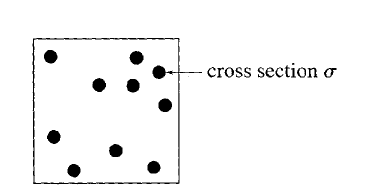
\includegraphics[width=0.2\textwidth]{targets.PNG}
	\end{figure}
	\item Probability that any one projectile hits one of these targets is
	\begin{align}
		P(\text{hit}) &= \dfrac{\text{total area of targets}}{total area} \\
		&= \dfrac{n_{tar} A \sigma}{A} = n_{tar} \sigma 
	\end{align}
	where $n_{tar}$ is \blue{number (area) density} = number of targets per unit area. 
	
	\item Then number of scattered particles if we send some number $N_{in}$ in is
	\graybox{N_{sc} = N_{inc} n_{tar} \sigma \tlab{14.2}} 
	which, in practice, is used to solve for the cross section $\sigma$, since this is usually the unknown.
	
	\item Nuclear cross sections are usually given in units of \blue{barn}, where
	\begin{align}
		1\text{ barn} &= 10^{-28} ~ m^2
	\end{align} 
\end{itemize}

\subsection{\green{Generalizations of $\sigma$ (14.3)}}
\begin{itemize}
	\item \Part{Scattering of Two Hard Spheres}. 
	\begin{itemize}
		\item They hit iff $b \le R_1 + R_2$. 	\myfig{sphere_scatter.PNG}
		\item Center of projectile must lie inside circle with area $\sigma = \pi (R_1 + R_2)^2$. Lesson: $\sigma$ is a property of the target and projectile and should be thought of as the effective area
		of the former for scattering the latter. 
	\end{itemize}
	
	\item \blue{elastic:} internal motions of target are left unchanged, else called \blue{inelastic.}
	
	\item \Part{Differential Scattering Cross Section}. 
	\begin{itemize}
		\item Setup: beam along $z$-axis. Directions of particles given by $\theta$ and $\phi$. Want to know number of particles in some cone around ($\theta, \phi$). 
		\item \blue{Solid angle} defined as subtending area $A$ on sphere of radius $r$:
		\graybox{\Delta\Omega &= A/r^2 \tlab{14.14} \\ d\Omega &= \sin\theta d\theta d\phi \tlab{14.15}}
	
		
		\item Define corresponding \blue{differential scattering cross section} as effective cross-sectional area of target for scattering into $d\Omega$, often written as \[
		d\sigma = \deriv{\sigma}{\Omega} d\Omega
		\]
		
		\item The number of particles scattered into $d\Omega$ can then be given by 
		\graybox{N_{sc} = N_{inc}n_{tar} \deriv{\sigma}{\Omega} d\Omega \tlab{14.17}}
		where the differential cross section is typically a function of $\theta ,\phi$. 
	\end{itemize}
\end{itemize}

	
\subsection{\green{Differential Cross Section (14.5)}}
\begin{itemize}
\myfig{HardSphere.PNG}
\item Independent of $\phi$ if axially symmetric. Want scattering angle $\theta$ as a function of $b$, or vice-versa. 

\item For picture above, $b = R\sin\alpha$ and $\theta = \pi - 2\alpha$

\item Particles incident between $b$ and $b + db$ that emerge between $\theta$ and $\theta + d\theta$ have 
\begin{align}
	d\sigma &= 2\pi b db \tlab{14.21} \\
	d\Omega &= 2\pi \sin\theta d\theta \tlab{14.22}
\end{align}
which means we can divide the two to get the differential cross section as
\graybox{\deriv{\sigma}{\Omega} = \dfrac{b}{\sin\theta}|\deriv{b}{\theta}| \tlab{14.23}}

\item To get diff cross section: (1) find $\theta(b)$ or $b(\theta)$, then (2) take derivatives. 


\end{itemize}

\subsection{\green{Rutherford Scattering}}
\begin{itemize}
	\item Scattering $\alpha$ particles off gold nuclei. Force on charge $q$ from nucleus is 
	\begin{align}
	F = \frac{kqQ}{r^2} = \frac{\gamma}{r^2} \tlab{14.26}
	\end{align}
	and so the ``orbit'' of the alpha is a hyperbola with nucleus at its focus, shown below. 
	
	\myfig{Rutherford.PNG}
	\myfig{RutherfordTriangle.PNG}
	
	\item Orbit is symmetric about DCA intersected by $\bm{u}$. Label position of particle by $\psi$, the angle from $\bm{u}$, which approaches limit $\psi \rightarrow \psi_0$ as particle moves away\footnote{Because symmetric, also have that $\psi \rightarrow -\psi_0$ as $t \rightarrow -\infty$}. Then
	\begin{align}
	\theta = \pi - 2\psi_0 \tlab{14.27}
	\end{align}
	since $2\psi_0$ is angle from horizontal (left) to eventual $p'$ in figure. 
	
	\item Math derivation with no explanations\footnote{Srsly just see where I bookmarked the pdf.}: 
	\begin{align}
		\Delta\bm{p} &= \bm{p'} - \bm{p} \tlab{14.28} \\
		|\Delta\bm{p}| &= 2p \sin(\theta/2) \tlab{14.29} \\
		|\Delta\bm{p}| &= \int_{-\infty}^{\infty} F_u dt \\
		&= \int_{-\psi_0}^{\psi_0}  \frac{\gamma\cos\psi}{r^2}\frac{d\psi}{bp/mr^2} = \frac{2\gamma m}{bp}\cos(\theta/2) \tlab{14.30} \\
		b &= \frac{\gamma}{mv^2}\cot(\theta/2) \tlab{14.31} 
	\end{align}
	
	\item \blue{Rutherford scattering formula}:
	\graybox{\deriv{\sigma}{\Omega} = \bigg( \dfrac{kq Q}{4 E \sin^2(\theta/2) }\bigg)^2 \tlab{14.32}}
	where $E$ is incident projectile energy $\onehalf m v^2$. 
	
	\newpage
	\Part{Example 14.6: Angular Dependence}
	\begin{itemize}
		\item Goal: To write eq~\ref{14.32} as
		\begin{align}
			\deriv{\sigma}{\Omega}(\theta) = \dfrac{\sigma_0(E)}{\sin^4(\theta/2) } \tlab{14.33}
		\end{align}
	\end{itemize}
\end{itemize}

\subsection{Cross Section in Various Frames}

\begin{itemize}
	\item CM frame: projectile and target approach each other with equal/opposite momenta. 
	\item Lab frame: Can be fixed target or both moving in opposite directions; In all cases the initial momenta are \textit{collinear}. 
	\item I'll save you time: All quantities individually in eq~\ref{14.2} are equal regardless of which frame (CM/lab) you're in. \begin{footnotesize} Equation~\ref{14.2} applies in either frame:
	\begin{align}
		N_{sc}^{cm} = N_{inc}^{cm} n_{tar}^{cm} \sigma_{cm}  \\
		N_{sc}^{lab} = N_{inc}^{lab} n_{tar}^{lab} \sigma_{lab}
	\end{align}
	where, if you aren't an idiot, you should be able to reason that $N_{sc}^{cm} = N_{sc}^{lab}$ and similarly that $N_{inc}^{cm} = N_{inc}^{lab}$  \end{footnotesize}

	\item Acknowledging that $\theta$ may differ between reference frames, the following is true in either:
	\begin{align}
		N_{sc}(\text{into d$\Omega$}) = N_{inc} n_{tar} \deriv{\sigma}{\Omega} d\Omega
	\end{align}
	
	\item The differential cross sections are \emph{not} the same in either frame, but only because $d\Omega_{cm}$ is not necessarily equal to $d\Omega_{lab}$. 
	\begin{align}
		\bigg(\deriv{\sigma}{\Omega}\bigg)_{lab} = \bigg(\deriv{\sigma}{\Omega}\bigg)_{cm}\deriv{\Omega_{cm}}{\Omega_{lab}}
	\end{align}
	and since $d\Omega = \sin\theta d\theta d\phi = -d(\cos\theta)d\phi$ where $\phi$ is same in either frame,
	\graybox{ \bigg(\deriv{\sigma}{\Omega}\bigg)_{lab} = \bigg(\deriv{\sigma}{\Omega}\bigg)_{cm}\deriv{(\cos\theta_{cm})}{(\cos\theta_{lab})}\tlab{14.45}}
\end{itemize}

% ==================================================================
%===================================================================
% CHAPTER 16 Continuum Mechanics
% ==================================================================
% ==================================================================
\clearpage
\twocolumn[
\begin{@twocolumnfalse}
	\sexin{Continuum Mechanics (Ch. 16)}
\end{@twocolumnfalse}]

\subsection{Transverse Motion of Taut String (16.1)}

\p \blue{1-D Wave Equation.} The usual derivation. Let $u(x,t)$ denote the vertical displacement of the string at point $x$ at time $t$, then the equation of motion of the string is
\graybox{
	\ppderiv{u}{t} &= c^2 \ppderiv{u}{x} \tlab{16.4}\\
	c &= \sqrt{\frac{T}{\mu}}\tlab{16.5}
	}
\p where $T$ is the tension in our string\footnote{Assumed constant across the string (unreasonable assumption imo).} and $\mu$ is its linear mass density. 

\myspace
\subsection{The Wave Equation (16.2)}

\p There are \textit{only} 3 kinds of solutions for $u$ in ~\ref{16.4}:
\begin{enumerate}
	\item A disturbance $u(x,t)$ that travels rigidly along string from left to right.
	\item `` \textellipsis\textellipsis '' right to left.
	\item Any combination of these two.
\end{enumerate}
and I'll sketch the main steps of the proof as follows. Change $x$ and $t$ to 
\begin{align}
	\xi = x - ct \qquad\quad \eta= x+ ct \tlab{16.6}
\end{align}
and we end up finding that the general solution ~\ref{16.4} must have the form
\graybox{
	u &= f(\xi) + g(\eta) \tlab{16.9} \\
	u(x, t) &= f(x - ct) + g(x+ct) \tlab{16.10}}
\p \red{Note:} $u(x, t)$ is a function of \textit{two} variables, but don't forget that both $f$ and $g$ only have single argument!

\myspace 
\Needspace{20\baselineskip}
\p \blue{Example 16.1: Triangular Wave}. A short segment of taut string has initial displacement $u(x, 0) = u_0(x)$. \textbf{Goal}: Find the disturbance $u(x, t)$ for any later time $t$. 
\begin{compactitem}
	\item \textbf{Initial displacement}. Can determine\textit{sum} of $f$ and $g$ (see ~\ref{16.10}) from initial conditions: $f(x) + g(x) = u_0(x)$. 
	\item \textbf{Initial velocity}. Note: the string is released \textit{from rest}.
	\begin{align}
	\begin{split}
		\left[ \pderiv{u}{t}\right]_{t = 0} &= -c \deriv{f(x)}{x} + c \deriv{g(x)}{x} = 0  \\
		f(x) - g(x) &= 0
	\end{split} \tlab{16.14}\\
	f(x) = g(x) = \onehalf u_0(x)
	\end{align}
	\item \textbf{Result}. The actual disturbance at any time $t$ is thus
	\begin{align}
		u(x, t) &= f(x - ct) + g(x + ct) = \onehalf u_0(x - ct) + \onehalf u_0(x + ct)\tlab{16.15}
	\end{align}
	\myfig[0.25\textwidth]{TriangleWave.PNG}
\end{compactitem}

\myspace
\p \blue{Standing Waves}. A special case is when $f$ and $g$ are sinusoidal. 
\begin{align}
u(x, t) = A\sin(kx - \omega t) + A\sin(kx + \omega t) = 2A\sin(kx)\cos(\omega t)\tlab{16.18}
\end{align}
This is not traveling left/right; it simply oscillates up and down like $\cos(\omega t)$ with amplitude (at any one point $x$) equal to $2A\sin(kx)$. In particular, at locations with $kx = n\pi$, we have \textbf{nodes}, positions that don't move at all. 

\myspace 
\subsection{Boundary Conditions Finite String (16.3)}

\begin{align}
u(0, t) &= u(L, t) = 0 \tlab{16.20} \\
u(x, t) &= X(x)\cos(\omega t - \delta) \tlab{16.21} \\
\dderiv{X(x)}{x} &= -k^2 X(x) \tlab{16.22} \\
u(x, t) &= \sin(kx)A\cos(\omega t - \delta) \tlab{16.26} \\
k &= k_n  = n\frac{\pi}{L} \quad [n = 1,2,3,\ldots]\tlab{16.27} \\
\omega &= \omega_n  = n\frac{\pi c}{L} \quad [n = 1,2,3,\ldots]\tlab{16.28}
\end{align}
where the individual solutions corresponding to $\omega_n$ are called the \green{harmonics}. The solution with $\omega_1$ is called the \green{fundamental} and successive modes are called \green{overtones}. \\

\p The main takeaway is that any possible motion can be written as a linear combination of the normal-mode solutions:
\graybox{
	u(x, t) &= \sum_{n = 1}^{\infty} \sin(k_n x) \left( B_n \cos(\omega_n t) + C_n \sin(\omega_n t) \right) \tlab{16.30}
	}
	
\myspace
\subsection{3-D Wave Equation (16.4)}

\p Let $p = p(x, y, z, t) = p(\bm{r}, t)$ denote some disturbance in a 3D system. Then the \textbf{3D wave equation} is
\graybox{
	\dderiv{p}{t} &= c^2 \nabla^2 p \tlab{16.39}}
\p where $\nabla^2 = \nabla \cdot \nabla$ is the \textbf{Laplacian}.

\myspace
\p \blue{Plane Waves}. If $\bm{n}$ denote arbitrary unit vector, then a disturbance of the form 
\begin{align}
	p &= f(\bm{n}\cdot\bm{r} - ct) \tlab{16.40} 
\end{align}
is const in any plane perp to $\bm{n}$ and travels in direction $\bm{n}$ with speed $c$. 

\myspace
\p \blue{Spherical Waves}


% ==================================================================
%===================================================================
% CENTER OF MASS BOOT CAMP
% ==================================================================
% ==================================================================
\clearpage
\twocolumn[
\begin{@twocolumnfalse}
	\sexin{Center of Mass}
	\begin{center} Review of CM-related material. \end{center}
\end{@twocolumnfalse}]

\p The \blue{center of mass} of a system of $N$ particles is a mass-weighted position average of the constitutent particles. The total momentum of the system can also be written in terms of the CM position.
\begin{align}
	\bm{R} 		&= \dfrac{m_1\R_1 + \cdots + m_N \R_N}{M} ~~ \mgreen{DISCRETE} \\
				&= \frac{1}{M}\int \rho \R dV ~~ \mgreen{CONT.}\\
	\bm{P} 		&= \sum_\alpha m_\alpha \R_\alpha = M \dot{\bm{R}} \\
	\F^{ext} 	&= M\ddot{\bm{R}} = \dot{\bm{P}}
\end{align}
\myspace

\p It is always true that, if the external torque $\bm{\Gamma}^{ext}$ about the CM is zero, then the total angular momentum $\bm{L}$ about the CM is conserved. \myspace

\p The \blue{CM frame} is the inertial frame in which the CM is at rest, i.e. that $\dot{\bm{R}} = 0$. 


% ==================================================================
%===================================================================
% Final Studying FML
% ==================================================================
% ==================================================================
\clearpage
\twocolumn[
\begin{@twocolumnfalse}
	\sexin{Final Stuff}
	\begin{center} Placing my questions here to come back to and answer later. \end{center}
\end{@twocolumnfalse}]

\p \blue{Main Ideas}
\begin{itemize}
	\item \textbf{Scattering}. To find the differential cross section $\sigma(\theta)$, find $\theta(b)$ or $b(\theta)$, and use to calculate
	\begin{align}
		\sigma(\theta) = \deriv{\sigma}{\Omega} = \frac{b}{\sin\theta} \bigg| \deriv{b}{\theta} \bigg|
	\end{align}
\end{itemize}

\myspace
\p \blue{Useful Equations}:
\begin{compactitem}
	\item Rolling w/o slipping: $T = \onehalf m v_{cm}^2 + \onehalf I_{cm} \omega^2$
	\item Moments of inertia: \myfig{InertiaList.PNG}
	\item \green{Perpendicular Axis Theorem}. For a body in the xy-plane, the perpendicular axis theorem states that $I_z = I_x + I_y$. 
	\item \green{Parallel Axis Theorem}. $I_{par} = I_{cm} + Md^2$. 
	\item \textbf{Solutions to common ODEs}:
	\begin{compactitem}[--]
		\item ODE: $ \ddot x + \omega_0^2 x = 0$; with (equivalent) general solutions:
		\begin{align}
			x(t) &= C_1 e^{i\omega t} + C_2 e^{ - i\omega t} \\
			x(t) &= B_1 \cos(\omega t) + B_2 \sin(\omega t) \\
			x(t) &= A\cos(\omega t - \delta)
		\end{align}
		
		\item ODE: $ \ddot x + 2 \beta\dot x + \omega_0^2 x = 0$; with general solution:
		\begin{align}
			x(t) &= e^{- \beta t} \left(C_1 e^{\sqrt{\beta^2 - \omega_0^2} t} +  C_2 e^{-\sqrt{\beta^2 - \omega_0^2} t}\right)
		\end{align}
		
		\item ODE: $ \ddot x + 2 \beta\dot x + \omega_0^2 x = f(t)$; with general solution:
		\begin{align}
			x(t) &= e^{- \beta t} \left(C_1 e^{\sqrt{\beta^2 - \omega_0^2} t} +  C_2 e^{-\sqrt{\beta^2 - \omega_0^2} t}\right)
		\end{align}
	\end{compactitem}
\end{compactitem}

\myspace
\p \blue{General Problem-Solving Skills}
\begin{compactitem}
	\item Be careful: $T = T_{rot} + T_{trans}$, e.g. if a thin rod is rotating about its end (which is fixed on ground), then $T = T_{rot}$ only. 
	\item Instead of finding equations of mot. via $\mathcal L$, GSI also employed energy conservation to write a general expression for $E$, and then solve $\deriv{E}{t} = 0$ for variables of interest.
	\item Knowing what general coordinates to use. 
	\item Finding and solving $\mathcal L$ for a system. 
	\item Frequency of small oscillations skills. 
	\begin{compactitem}[$\oplus$]
		\item At equilibrium, $\dot \theta = \ddot \theta = 0$. This tells us info about $\theta_{eq}$. 
		\item To find small osc $\dot \theta$, plug back in $\theta_{eq} + \epsilon$ in E.O.M. and solve. 
	\end{compactitem}
	
	\item Principal axes can be easily found by considering the body's symmetry. E.g. for a square it is by placing origin at center of square. 
	\item The moment of inertia tensor $I$ is defined with respect to some \textit{origin} (relative to body). Therefore, when just switching axes, don't forget that you can still use the same $I$ tensor applied to the direction $\omega$ to determine $L = I \omega$. 
\end{compactitem}





\clearpage
\twocolumn[
\begin{@twocolumnfalse}
\sexin{Formula Dump}
\end{@twocolumnfalse}]
\setlength{\columnseprule}{0pt}


\subsubsection{Coordinate Systems}

\begin{table}[h]
	\centering
	\begin{tabular}[c]{L L}
		\toprule\toprule
		\text{Cartesian} 	& \text{Polar} \\
		x = r \cos\phi 		& r = \sqrt{x^2 + y^2} \\
		y = r \sin\phi		& \phi = \arctan(y/x) \\
		\F = m\bm{a} 		& \F = m( \ddot{r} - r \dot{\phi}^2)\hat{\R} + m(r \ddot{\phi} + 2 \dot{r} \dot{\phi} ) \hat{\bm{\phi}}\\
		\bottomrule\bottomrule
		% --------------------------------------------------------------------------------
		\text{Polar Vectors} & \text{Polar Derivatives} \\
		\R = r \hat{\R}  	& \deriv{\hat{\R}}{t} = \dot{\phi}\hat{\bm{\phi}} \\
		\dot{\R} = \dot{r}\hat{\R} + r\dot{\phi}\hat{\bm{\phi}} & \deriv{\hat{\phi}}{t} = -\dot{\phi}\hat{\R} \\
		\ddot{\R} = \big( \ddot{r} - r \dot{\phi}^2 \big)\hat{\R} + \big(r \ddot{\phi} + 2 \dot{r} \dot{\phi} \big) \hat{\bm{\phi}} &\\
		\bottomrule\bottomrule
		% --------------------------------------------------------------------------------
		\text{Spherical Polar Coordinates} 	& \text{Cylindrical Polar}	\\ 
		x = r\sin\theta\cos\phi 			& d\bm s = d\rho \hat{\bm{\rho}} + \rho d\phi \hat{\bm{\phi}} + dz \hat{\bm{z}}	\\
		y = r\sin\theta\sin\phi 			& \nabla \equiv \hat{\bm{\rho}} \pderiv{}{\rho} + \hat{\bm \phi} \frac{1}{\rho} \pderiv{}{\phi} + \hat{\bm{z}} \deriv{}{z}\\
		z = r\cos\theta 					& \bm{\dot \rho} = \dot \rho \hat{\bm \rho} + \rho \dot{\phi} \hat{\bm{\phi}}	 + \dot z \hat{\bm{ z}}			\\
		d\R = dr \hat{\R} 
		+ rd\theta
		 \hat{\bm{\theta}} 
		+ r\sin\theta 
		d\phi \hat{\bm{\phi}} 				& \\
		\nabla f = 
		\rhat \pderiv{f}{r} 
		+ 
		\thetahat \frac{1}{r} 
		\pderiv{f}{\theta} 
		+ \phihat \frac{1}{r\sin\theta}  
		\pderiv{f}{\phi}
	\end{tabular}
\end{table}

\subsubsection{Ellipse}
\begin{itemize}
	\item Equation of an ellipse whose major axis is the x-axis and minor axis is the y-axis (a>b):
	\begin{align}
		\bigg(\frac{x-h}{a}\bigg)^2 + \bigg(\frac{y-k}{b}\bigg)^2 = 1
	\end{align}
	where (h, k) is the center of the ellipse. 
	\item Parametric formula:
	\begin{align}
		x(t) &= a \cos t \\
		y(t) &= b \sin t 
	\end{align}
\end{itemize}

\clearpage
\subsubsection{ODE Stuff}
\begin{itemize}
	\item The \blue{Laplace transform} of a function defined for $t \ge 0$ is defined as 
	\begin{align}
		\mathcal{L}\{f(t)\} = \int_0^\infty e^{-st} f(t) dt \equiv F(s)
	\end{align}
	\item Let $y = \sin at$ for $t > 0$ else 0. 
	\begin{align}
		\mathcal{L}\{y(t)\} = \int_0^\infty e^{-pt} \sin( at) dt = \frac{p}{p^2 + a^2}
	\end{align}
	\item Let $y = g(t-a)$ for $t > a > 0$ else 0. 
	\begin{align}
	\mathcal{L}\{y(t)\} = \int_a^\infty e^{-pt} g(t-a)  dt = e^{-pa}  G(p)
	\end{align}
\end{itemize}

\subsubsection{Trig Identities}
\begin{compactitem}[$\rightarrow$]
	\item  Double-angle formulas. 
	\begin{align}
		cos(2u) &= cos^2u - sin^2u  \\
		&= 2cos^2u - 1 \\
		&= 1 - sin^2u
	\end{align}
	\begin{align}
	tan(2u) = \frac{2tanu}{1 - tan^2u}
	\end{align}
	
	\item Half-angle formulas. 
	\begin{align}
		sin^2u &= \frac{1 - cos(2u)}{2} \\
		cos^2u &= \frac{1 + cos(2u)}{2}
	\end{align}
\end{compactitem}


\clearpage
\twocolumn[
\begin{@twocolumnfalse}
	\sexin{Lecture Notes}
\end{@twocolumnfalse}]
\setlength{\columnseprule}{0.2pt}

\subsection{\green{Orbits Oct 3}}
\begin{itemize}
	\item Planets move in elliptical orbits:
	\begin{align}
		\frac{\alpha}{r} &= 1 + \epsilon \cos\theta \\
		\alpha &= a(1-\epsilon^2) \\
		b^2 &= a^2(1-\epsilon^2)
	\end{align}
	\item Precession of planetary orbits. 
	\item $\delta = 3GM_0 / c^2 << 1$. 
	\item Since $\delta << 1$, solution resembles ellipse:
	\begin{align}
		u = \frac{1}{\alpha}(1 + \epsilon cos\theta) - \delta u_1 + \cdots 
	\end{align}
	\item Expands out a ton of Taylor series. 
	\item Moving on to scattering. Particularly hyperbolic motion when scattering in 1/r potential 
	\item Elastic collisions: 
	\begin{itemize}
		\item No energy loss. 
		\item Let $u_1$, $u_2$ be initial velocities in lab frame; $v_1$, $v_2$ the final velocities in lab frame. 
		\item Easier to solve in CM frame. Prime quantities in this frame. 
	\end{itemize}
\end{itemize}


\subsection{oct 10}
\begin{itemize}
	\item cross-section for scattering in CM frame. 
	\begin{align}
		\sigma(\theta) = \frac{b}{\sin\theta}\deriv{b}{\theta}
	\end{align}
	\item In CM frame
	\begin{align}
		\ell &= \mu \mu' b \\
		&= b \sqrt{2 \mu E}
	\end{align}
	since $E = \onehalf \mu \mu'^2$. 
	
	\item Since $\theta = \pi - 2\Theta$, need to calculate first:
	\begin{align}
		\Theta &= \int \dot{\Theta} dt \\
		&= \int \hat{\Theta} dr/\dot{r} \\
		&= \int \dfrac{(\ell/\mu r^2) dr}{\sqrt{2/\mu (E - U(r) - \ell^2/2\mu r^2)}}
	\end{align}
	
	\item \blue{Rutherford scattering formula:}
	\begin{itemize}
		\item Suppose $U(r) = k/r$. If $k < 0$, attracting; else repelling. 
		\item Have 
		\begin{align}
				\Theta &= \int_{r_{min}}^\infty \dfrac{(b/ r^2) dr}{\sqrt{1 - 2\kappa/r - b^2/r^2}}
		\end{align}
		where $\kappa = \onehalf k/E$. 
		\item Let $r = b/u$ and write integral in terms of u. 
		\begin{align}
			\Theta &=\int_{b/r_{min}}^0 \dfrac{(u^2/ b) (-b/u^2)du}{\sqrt{1 - 2\kappa u/b - u^2}} \\
			&\int \dfrac{du}{1 + \kappa^2/b^2 - (u + \kappa/b)^2}
		\end{align}
		\item Now substitute $u + \kappa/b = \sqrt{1 + \kappa/b^2} \cos\alpha$ where $\alpha$ is a new variable.
		
			 
		\begin{align}
			\Theta &= \dfrac{ \sqrt{1 + \kappa/b^2} (-\sin\alpha)d\alpha}{ \sqrt{1 + \kappa/b^2} \sin\alpha} \\
			&= \alpha
		\end{align}
		
		\item Result is 
		\begin{align}
			\cos\Theta &= \dfrac{\kappa}{\sqrt{\kappa^2 + b^2}} \\
			&= \sin(\Theta/2)
		\end{align}
	\end{itemize}
\end{itemize}

\newpage
\subsection{Oct 12}
\begin{itemize}
	\item From last lecture, know that i CM frame, 
	\begin{align}
		\sigma = \frac{\kappa^2}{4 \sin^4(\theta/2)}
	\end{align}
	where $\theta$ is angle in CM frame and $\kappa = k/2E$. 
	
	\item \Part{Dynamics in rotating frames:}
	\begin{itemize}
		\item Want expression for acceleration
		\begin{align}
		 \deriv{r}{t}|_{intertial} &=  \deriv{r}{t}|_{rotating} + \omega \times r \\
		 \deriv{^2 r}{t^2}_{intertial} &= \deriv{^2 r}{t^2}_{rotating} + 2 \omega x \deriv{ r}{t}_{rot}  + \dot{\omega} \times r + \omega \times (\omega \times r) \\
		 &= F/m \\
		 \deriv{^2 r}{t^2}_{rot}&= F/m - 2 \omega \times v|_{rot} - \dot{\omega} \times r - \omega \times (\omega \times r) 
		 \end{align}
		 where last three terms are Coriolis force, azimuthal force, centrifugal force. 
	\end{itemize}
	
	\Part{Motion on a turntable}
	\begin{itemize}
		\item Assume $\omega$ is constant. Draw a circle centered in xy plane. Radial motion in rotating frame.
		\item $v = v e_x$ (unit vector e) $r = x e_x$. 
		\item Effective force
		\begin{align}
			F_{eff} &= -m \omega \times (\omega \times r) - 2m \omega \times v \\
			&= -m\omega^2 e_z \times ( e_z \times e_x) - 2m \omega v e_z \times e_x \\
			&= -m\omega^2 (-e_x) - 2m\omega v e_y 
		\end{align}
		
		\item if particle is moving in y direction on turntable $v = v e_y$, then
		\begin{align}
			F_{eff} &= m \omega^2 x e_x + 2 m \omega v e_x
		\end{align}
		so the forces are now in the same direction. 
	\end{itemize}
	
	\Part{Motion relative to Earth}
	\begin{itemize}
		\item Effect of earth is actually rotating?
		\item $r = R + r'$ where $R$ is origin of my rotating coordinate system and $r'$ is measured relative to that. 
		\item newton's second law
		\begin{align}
			m\rddot' &= F_{inert} - 2\omega \times \rdot' - m \dot{\omega }\times (R + r') - m \omega \times ( \omega \times (R + r')) \\
			&= F_{inert} - 2m \omega \times \rdot - m \dot{\omega} \times R - m \omega \times (\omega \times R) \\
			&= mg' - 2m\omega\times\dot{r}'
		\end{align}
		where $g'$ is now the effective gravitational acceleration. 
	\end{itemize}
	
	\item $t = \sqrt{2h/g'}$ for particle in free-fall deflection from Coriolis force. $\ddot{x} = 2\omega g' t\cos\lambda$. 
	
\end{itemize}



\newpage
\subsection{Lagrangian examples Oct 21}


\p \blue{Example: spring pendulum}. Natural length $l$ and spring const $k$. 
\begin{align}
	T &= \onehalf m (\rdot^2 + r^2 \dot{\theta}^2) \\
 U &= -mgr\cos\theta + \onehalf k (r - l)^2 \\
 \mathcal{L} &=  \onehalf m (\rdot^2 + r^2 \dot{\theta}^2) + mgr\cos\theta + \onehalf k (r - l)^2 
\end{align}
then take derivatives to get Lagrange equations. \\ \\

\p \blue{Example: Pendulum with moving vertical support}. Pendulum origin moving up. Apparently only one degree of freedom still, since $\zeta(t)$ (vertical) is known  
\begin{align}
	T &=	\onehalf m \bigg[ \big(l \dot{\theta}\cos\theta\big)^2 + (l\dot{\theta}\sin\theta + \dot{\zeta})^2 \bigg]  \\
	&= \onehalf m \bigg[ \big(l^2\dot{\theta}^2 + 2 (l\dot{\theta} \dot{\zeta}\sin\theta) +2\dot{\zeta}^2\bigg] \\
	% -------------------------
	U &= -mgl\cos\theta + mg\zeta(t) \\
	\mathcal{L}(\theta, \dot{\theta}) &= \onehalf m \bigg[ \big(l^2\dot{\theta}^2 + 2 (l\dot{\theta} \dot{\zeta}\sin\theta) +2\dot{\zeta}^2\bigg] +mgl\cos\theta - mg\zeta(t)  
\end{align} 
then take derivatives and stuff. Result is 
\graybox{l\ddot{\theta} + (g + \ddot{\zeta})\sin\theta = 0}
\p Note: effect of accelerating up is something something gravity something something equivalence principle. \\ \\

\p \blue{Now attach pendulum to spring}. Phase space variables now are $(\zeta, \theta, \dot{\zeta}, \dot{\theta})$. 
\begin{align}
	T &= \onehalf m \bigg[ l^2\dot{\theta}^2 + 2 (l\dot{\theta} \dot{\zeta}\sin\theta) +2\dot{\zeta}^2\bigg] \\
	% -------------------------
	U &= -mgl\cos\theta + mg\zeta(t) + \onehalf k (\zeta - \zeta_0)^2 
\end{align}
which is basically same as before.  \\ \\

\p \textbf{\blue{Mathieu equation}}. Suppose $\zeta(t)$ is given and $\zeta = a \cos\Omega t$ is position of support of pendulum [moves in sinusoidal way]. Then we have to solve
\begin{align}
\ddot{\theta} + (\alpha + \beta\cos t) \theta = 0
\end{align}
which is the \textbf{Mathieu equation}. Not a constant coefficient problem. Can't look for solutions that go like $e^{-t}$ or anything like that. $\alpha$ is square of natural frequency of oscillator. Each time pendulum goes through $\theta = 0$, the tension is largest. Suppose exactly at that time, we are raising the mass. Then we are doing \textit{work} on the mass. Suppose oscillation of support movement is twice the oscillation of $\sqrt{\alpha}$. We are putting enery in the system every cycle then. Therefore, \textbf{unstable solution} however small $\beta$ is, as long as it is not zero. This is simple model for parametric instability. 










\end{document}
